\begin{quote} ``Just as the constant increase of entropy is the basic law of the universe, so it is the basic law of life to be ever more highly structured and to struggle against entropy'' - \textit{Vaclav Havel}  \end{quote} 
 
While our previous chapter discussed the impact of data integration of the same type (microarrays), in this chapter we focus on the integration of the other type, where datasets of different types are used in a cooperative manner. Different datasets are not being merged \textit{literally}, but one is used to \textit{guide} the clustering of the other. We propose a type of clustering method with \textit{supervision} extracted from \textit{prior biological knowledge} in order to guide the process of clustering.

When a small amount of prior knowledge is available in the form of \textit{pairwise relationships} between genes, instead of simply using this knowledge for the external validation of the results of clustering, we can use it in order to guide the clustering process thus providing a limited form of supervision. We call these methods \textit{semi-supervised clustering} \footnote{This is different from Semi-Supervised Learning \citep{grira2005unsupsurvey} which is a class of machine learning techniques that make use of both labelled and unlabelled data for training. They are called semi-supervised because the available knowledge is far from being enough for fully supervised learning even in a transductive form.} because unlike supervised or constrained clustering \citep{bradley00constrained}, the final results of clustering is not required to enforce the constraints. The constraints act as guidelines and are enforced only if they are complementary to the data being clustered. For semi-supervised clustering to be profitable, the two sources of information, i.e., the similarity measure (used by all clustering methods) as well as the constraints available should not completely contradict each other.
In our novel formulation, named \acfi{SSSC}, supervision (prior knowledge) is provided in the form of binary constraints and clustering is done in the spectral space \citep{shi00normalized, ng2001onspectral}. The prior knowledge is derived from DNA binding data from ChIP-chip experiments, PPI data and known TF-gene interactions from a curated database. These are used to guide the process of clustering microarray data.

\section{Spectral Clustering}
The goal of any clustering is to partition a set of points into disjoint sets where the points within a partition are as similar as possible while points within different partitions are as dissimilar as possible. In this section, we discuss how spectral clustering achieves this objective. 
\subsection{Graph notations}
Given a set of data points, we can compute similarities between them using a suitable \textit{similarity function}. Given these similarities between the data points, a dataset can be represented as a \textit{graph} which is a set of \textit{vertices} and \textit{edges} connecting vertices \textit{(V,E)}. The vertices \textit{(V)} represent the data points while the edges \textit{(E)} represent the links between the data points. Usually a certain threshold of similarity value is chosen above which the edges are linked between data points. For \textit{weighted} graphs the edges also have the similarity values as \textit{weights}. Once we have this undirected weighted graph, the goal of a clustering algorithm is to partition it such that edge weights between the points \textit{within} a partition are high while the edge weights between points of \textit{different} partitions are low. We begin with some definitions.

Let $G = (V,E)$ be an \textit{undirected weighted} graph with vertices $V = {v_{1},\dots,v_{n}}$, edges $E= {e_{1},\dots,e_{n}}$ and each edge $e_{ij}$ between vertex $i$ and $j$  has a non-negative weight $w_{ij}$. The weights matrix $W = (w_{ij})_{i,j=1,\dots,n}$ is also known as the \textit{adjacency matrix} of this graph. For non existing edges, $w_{ij}=0$. The graph is assumed to have no self-edges, i.e., $w_{ii}=0$. In order to understand spectral clustering we need some more definitions for this graph.

The \textit{degree} ($d_{i}$) of a vertex $v_{i}$ is defined as
\[
d_{i} = \sum_{j=1}^{n}w_{ij}
\]

which intuitively is the row-wise sum for the respective row of the adjacency matrix. In the graph, this can also be understood in terms of sum of edge weights for that particular vertex. The \textit{degree matrix} $D$ is defined as the \textit{diagonal} matrix with the individual vertex degrees $d_{1}$, \dots, $d_{n}$ along the diagonal, everything else being $0$.

\subsection{Similarity matrices and graph Laplacians}
There are various ways of converting similarities between a given set of data points into a graph - both in choosing the similarity function to compute similarities 
among the data points as well as deciding about how to turn the similarity values into a graph.

A \textit{$\varepsilon$-neighbourhood} graph is obtained by joining edges between points whose similarity values are larger than  $\varepsilon$. 
Figure-\ref{fig:constraints_with_pval} shows two examples of such a graph using two different values of $\varepsilon$. A \ac{KNN} graph has edges between a 
point and $k$ other points that are most similar to it. This leads to a directed graph because the neighbourhood relation is not 
symmetric, i.e., $v_{a}$ might have $v_{b}$ as one of its k-nearest neighbours but the vice-versa might not be true. To convert this into an 
undirected one, we can either totally ignore the direction or take a more restrictive approach where two nodes are connected \textit{only} if 
both of them are \aclp{KNN} of each other. The latter type is also referred to as a \textit{mutual \acl{KNN} graph}.

A \textit{fully connected} graph is one where all pairs of points have positive similarity values and are connected. This leads to a denser 
graph in comparison to previous ones. While in the earlier ones, the local neighbourhood relationship was enforced with either a 
threshold ($\varepsilon$) or a maximum of $k$-neighbours, in a fully connected graph we have to choose a similarity function that should 
do this. For all our work, we have used the Gaussian similarity function which encodes this neighbourhood relation automatically. 
In this function, $exp \left( -\frac{{\parallel \textbf{x}-\textbf{x}^{'} \parallel}^{2}}{2\sigma^{2}}\right)$, $\sigma$ controls the width of 
the neighbourhood and $\textbf{x}$,$\textbf{x}^{'}$ represent the two variables between which similarity is being computed. The Gaussian similarity 
function is an exponential function, therefore depending on $\sigma$, the similarity falls non-linearly 
(exponentially) with increasing distance. This property makes it desirable to use where neighbourhood relations are important. Various 
other similarity functions for vector data are discussed in Chapter-\ref{chap_maxent}.

Spectral clustering is based on the \textit{Laplacian} matrix which has its origins in spectral graph theory \citep{chung1997spectralgraph}. There are various types of Laplacians. All of these assume that we have an undirected graph $G$ with positive weight matrix $W$ ($w_{ij} \geq 0$) and a corresponding degree matrix $D$. An \textit{unnormalized} Laplacian is defined as 

\[
	L = D-W
\] 
The matrix $L$ has the following properties
\begin{itemize}
    \item $L$ is always symmetric and positive semi-definite.
    \item $L$ has $n$ non-negative, real-valued eigenvalues $\lambda_{1}(=0) \leq \lambda_{2}\leq \dots \leq \lambda_{n}$. The number of smallest eigenvalues (=0), i.e., its multiplicity, corresponds to the number of connected components in the graph. 
\end{itemize}

There are two popular variants of the \textit{normalized} Laplacian. They are defined as

\begin{eqnarray}
	L_{symmetric} &=& D^{-1/2} L D^{-1/2} = I - D^{-1/2} W D^{-1/2} \label{eqn-lap_sym}\\
	L_{random walk} &=& D^{-1}L = I - D^{-1}W 
\end{eqnarray}
where $D^{-1/2}$ is the inverse square root of matrix $D$. Since $D$ is a diagonal matrix and the square root of a diagonal matrix D is formed by taking the square root of all the entries on the diagonal

\begin{displaymath}
    \mathbf{D^{\frac{-1}{2}}} = \begin{bmatrix} \frac{1}{\sqrt{d_{11}}} & 0 & \dots & 0\\
				 0 & \frac{1}{\sqrt{d_{22}}} & \dots & 0\\
                                 \vdots & \vdots & \ddots & \vdots\\
				 0 & 0 & \dots & \frac{1}{\sqrt{d_{nn}}}\\
                 \end{bmatrix}
\end{displaymath}
Like the unnormalized Laplacian, the normalized ones are also always symmetric and positive semi-definite. They too have non-negative, real-valued 
eigenvalues $\lambda_{1}(=0) \leq \lambda_{2}\leq \dots \leq \lambda_{n}$ and the multiplicity of the smallest eigenvalue is the number of 
connected components in the graph. Laplacians could be interpreted as \textit{gradients} on graphs and it is related to differential geometry. 
\subsection{Graph clustering}
As seen earlier, given a set of data points, a similarity function can be used to calculate the pairwise similarities among them, resulting in a similarity matrix. Given its graph representation, the clustering can be defined as a \textit{graph partitioning} problem where the edges between the points of the \textit{same} cluster have high weights while the edges between points belonging to \textit{different} clusters have low weights. Before we discuss the algorithm in detail, we discuss the general problem of graph clustering and its relation to spectral clustering. 

We know that the key objective of clustering is to find sets of points that are \textit{maximally similar to each other within a set} 
and \textit{maximally dissimilar to points in other sets}. If we have a similarity graph, as discussed earlier, the problem can be restated to 
find a partition of the given graph such that the edges between points within a partition have higher weights as compared to edges 
between points in different partitions. Graph clustering or partitioning is an old problem 
and has been exhaustively studied \footnote{For a good review, see \cite{schaeffer1997graphclustering}}. Spectral clustering can be derived as an approximation to the graph partitioning objectives \citep{luxberg2006tutorial_spectral}. Before we start, we need some definitions.

If we have two disjoint partitions A, B then 
\[
	Cut(A,B) = \sum_{i \in A,j \in B}w_{ij}
\] 
	
So, if we have a graph G with adjacency matrix $W$, then we can construct a partition by solving the \textit{min-cut} problem, which can be understood 
as choosing the partitions $A_{1},\dots,A_{k}$ such that we minimize the following cut.

\[
	Cut(A_{1},\dots,A_{k}) = \sum_{i=1}^{k}Cut(A_{i},\bar{A}_{i})
\] 
where \={A} is the complement of $A$. While theoretically it can be solved, yet in practice it may yield clusters of 
size 1 (trivial clusters), which is not usually the goal of clustering. We want clusters that are \textit{reasonably} big. This is 
specified in terms of two popular \textit{objective functions} namely \textit{RatioCut} and normalized cut or \textit{NCut}.

\begin{eqnarray}
    RatioCut(A_{1},\dots,A_{k}) &=& \sum_{i=1}^{k}\frac{Cut(A_{i},\bar{A}_{i})}{|A_{i}|} \\
    NCut(A_{1},\dots,A_{k}) &=& \sum_{i=1}^{k}\frac{Cut(A_{i},\bar{A}_{i})}{vol(A_{i})}
\end{eqnarray}

While in RatioCut the normalizing factor is the $|A_{i}|$, which is the total number of vertices (points) in the $i_{th}$ partition, in NCut, the normalizing factor is $vol(A_{i})$ which is the sum of all edge weights in the partition. The role of this normalizing factor is to make the partition \textit{balanced} as measured by number of vertices or sum of edge weights. Even though the formulation is simple and elegant, it is an NP-hard\footnote{NP-hard (nondeterministic polynomial-time hard) is a class of problem in computational complexity theory} problem. The spectral clustering algorithm is a way to solve a relaxed version of these objective functions. 

Another way to understand this is that in both RatioCut and NCut, the numerator tries to achieve the objective of making different clusters as dissimilar to each other as possible, i.e., minimize the between cluster similarity. This is one half of the key requirement of any clustering algorithm's objective. The other half is that the within-cluster similarity should also be maximized. In other words $\sum_{i,j \in A}w_{ij}$ and $\sum_{i,j \in \bar{A}}w_{ij}$ should be maximized. Let's see how this is satisfied in each of the objective functions. 

\begin{eqnarray}
 \sum_{i,j \in A}w_{ij} &=& \sum_{i \in A, j \in A \cup \bar{A}}w_{ij} - \sum_{i \in A, j \in \bar{A}}w_{ij} \\
                        &=& vol(A) - Cut(A,\bar{A})	 
\end{eqnarray}

We can see that NCut satisfies this by maximizing $vol(A)$ and minimizing $Cut(A,\bar{A})$. RatioCut doesn't lead to this objective. As shown in \citet{luxberg2006tutorial_spectral}, relaxing NCut leads to using the \textit{normalized} Laplacian in spectral clustering while relaxing RatioCut leads to the use of \textit{unnormalized} Laplacian. Therefore, normalized spectral clustering satisfies both the key clustering criteria while unnormalized spectral clustering only implements the first criteria. One key point to note is that there is no guarantee on the quality of the clustering solution of the relaxed problem compared to the exact solution. 

\subsection{Algorithm explanation}
Spectral clustering is a technique in which the eigenvectors of the Laplacian matrix (which is derived from the \textit{similarity} matrix) corresponding to 
the smallest eigenvalues are used to derive a clustering of the given data points. The methods are called spectral, because 
they make use of the \textit{spectrum}\footnote{The set of eigenvectors of the normalized Laplacian matrix is usually called 
the \textit{spectrum} of the Laplacian (or the spectrum of the associated graph)} of the graph. It has been applied to diverse 
domains, e.g. image segmentation \citep{shi00normalized, weiss1999segmentation} and bioinformatics \citep{speer05spectral}. Most spectral clustering algorithms 
can be considered to have three stages:
\begin{description}
    \item[Normalization] This consists of computing the similarity matrix from the raw data using a suitable similarity function. We call this the \textit{normalization} step because different types of data (vector, graph or string) get converted to a common format (similarity matrix).
    \item[Eigen Decomposition] This consists of computing the eigenvalues and the corresponding eigenvectors of the similarity matrix. This step could be considered as the mapping of original data to the spectral domain.
    \item[Clustering] This step consists of using a traditional clustering algorithm (usually k-means) to cluster the vectors in the spectral domain.	
\end{description}
Different spectral clustering algorithms differ in the number of eigenvectors used (single or many) as well as the type of Laplacian 
used (unnormalized or normalized). \citet{verma2003comparison} did a systematic comparison of different popular 
spectral \citep{shi00normalized, ng2001onspectral, meila2000learning} and traditional clustering algorithms on artificial as well as 
real-world datasets. They report that spectral methods are more stable to noise than other tested algorithms. 
Both \citet{shi00normalized} and \citet{meila2000learning} have used the $L_{random walk}$ normalized Laplacian while \citet{ng2001onspectral} 
have used the $L_{symmetric}$ normalized Laplacian. Apart from this, there is no major difference between the techniques of all these algorithms. 
Since \citet{verma2003comparison} did not find significant differences among the two normalized Laplacians, we have used the 
algorithm by \citet{ng2001onspectral} which is the most recent one. This algorithm is described in Algorithm-\ref{alg:spectral_clustering}.
\begin{algorithm}
\caption{Spectral clustering}
\label{alg:spectral_clustering}
\begin{algorithmic}[1]
\REQUIRE Dataset ($X$), number of clusters ($k$) 

\STATE Calculate the symmetric similarity matrix $K_{n \times n}$  using Gaussian similarity function  $K_{ij}=exp \left( -\frac{{\parallel x_{i}-x_{j} \parallel}^{2}}{2\sigma^{2}}\right)$ if $i\neq j$, and set $K_{ii}=0$. 

\STATE Calculate normalized Laplacian $L'=D^{-1/2}KD^{-1/2}$ where D is the diagonal matrix with $d_{jj}=\sum_{i}d_{ji}$ 

\STATE Find the eigenvectors $v^{1},v^{2},\dots,v^{k}$ corresponding to the largest k eigenvalues of $L'$. 

\STATE Use these k eigenvectors as columns to get $V_{n \times k}$. 

\STATE Normalize the row to have unit norm, i.e., $U_{n \times k}$ such that $u_{ij}= v_{ij}/(\sum_{k}{v_{ik}^{2}})^{\frac{1}{2}}$

\STATE Cluster the points representing the rows of this matrix $(u_{i})_{i=1,...,n}$ using k-means algorithm into k clusters, $C_{1},C_{2},\dots,C_{k}$.  

\STATE Output clusters $A_{1},A_{2},\dots,A_{k}$ such that $A_{i}=\{x_{j}|u_{j}\in C_{i}\}$. This assigns the original point $x_{j}$ to cluster $A_{i}$ if $u_{j}$ is in cluster $C_{i}$. 

\end{algorithmic}
\end{algorithm}

In the previous description of this algorithm, we had mentioned that the eigenvectors corresponding to the smallest eigenvalues are used. However, in the step-3 of algorithm, we are proposing to take the eigenvectors corresponding to the largest k eigenvalues. This is because here we are using the Laplacian $L'$ instead of the form $L_{symmetric=}I-L'$ described earlier (refer eqn-\ref{eqn-lap_sym}). This changes the eigenvalues from $\lambda_{i}$ to $1-\lambda_{i}$.

To summarize the functioning of this algorithm: it changes the representation of the data points from the original space to the spectral space after the various steps (1-5) of transformation as shown in Algorithm-\ref{alg:spectral_clustering}. After that, any clustering algorithm can be used to cluster the data points. The reason for this transformation is that it allows better identification of non-linear clusters. Non-linear patterns are very hard to identify using traditional clustering methods but after the spatial transformation it becomes trivial to find them. For a detailed understanding of why this algorithm works, refer \citet{ng2001onspectral}. 

Spectral clustering is very appealing because it yields a very standard linear algebra problem for which there are various efficient solvers (algorithm implementations) already available. It can be implemented for even large datasets if the similarity matrix is sparse. Unlike traditional clustering algorithms like k-means, there are no issues of dependency on starting point or getting stuck in local optimum. On the flip side, choosing the right similarity function and its parameters is non-trivial.

\section{Datasets and Our Algorithm} \label{chap2:sec:materials}

\subsection{Microarray datasets}
We have used two popular microarray datasets on which the clustering is carried out, both of them based on experiments done on yeast (Saccharomyces cerevisiae). The dataset by \citet{gasch00genomicexpn} was obtained by exposing yeast to diverse environmental (stress) conditions such as temperature shocks, hydrogen peroxide, the superoxide generating drug menadione, the sulfhydryl-oxidizing agent diamide, the disulfide-reducing agent dithiothreitol, hyper and hypo-osmotic shock, amino-acid starvation and nitrogen source depletion. More than 900 genes showed drastic response to these environmental changes. We selected only those genes that displayed a change of three fold in \textit{at least one experiment}. There were 1246 genes fulfilling this criterion. The assumption behind this selection strategy is that the majority of genes which do not show much change in their expression levels during a process are unrelated to it.

The second microarray dataset was based on cell-cycle experiments by \citet{spellman98comprehensive} where the objective was to identify yeast genes which were involved in cell-cycle regulation. This was achieved using DNA microarrays synchronized using three independent methods: $\alpha$ factor arrest, elutriation, and arrest of a cdc15 temperature sensitive mutant. Again, we selected only those genes that displayed a change of two fold in \textit{at least one experiment}. There were 1732 genes fulfilling this criterion. The reason why we only filtered for two fold change is because stress leads to a much more widespread expression change across the genome. Therefore, the number of genes that show change at two fold are too high. On the other hand, expression level changes are not that severe in a normal cell-cycle study. So, the number of genes at two fold change are not that high.

In both the datasets, for data imputation we use the R \textit{impute} package which uses \textit{k-nearest neighbour} algorithm to impute missing values. It uses a Euclidean distance metric for finding nearest neighbours. We used the $log_{2}$ of the ratio of the mean of Channel 2 (experimental expression) to the mean of Channel 1 (control expression) since this is likely to create a Gaussian distribution \citep{ernstwit2004statis_microarrays}.

For the experiments where we combined microarray with DNA-binding data, we needed to do other steps of pre-processing. We found the list of genes responsible for the TFs that were tested for binding. Then we ensured that our microarray dataset had those. The reasoning behind this is that some of them might be missing after the filtering step. In such a case, they were extracted from the original unfiltered dataset and incorporated in the final filtered one. The number of these is small compared to the total number of genes and we didn't want to loose any of them.

\subsection{DNA-binding dataset}
One of the datasets which we have used to guide the clustering process is the DNA-binding dataset on yeast \citep{harbison04transcriptional}. It was created using genome-wide 
location analysis techniques to determine the genomic occupancy of 203 DNA-binding transcriptional factors. In this dataset, the likelihood of a particular TF 
binding to the promoter region of another gene is reported in terms of a confidence value (p-value). A lower p-value indicates higher confidence. In order to extract binary 
constraints from this dataset, we need some threshold on these reported p-values of interactions. We investigated a range of p-value cut-offs, each corresponding to a 
certain set of constraints. This was to study the impact of \textit{number} and \textit{quality} of constraints on the biological significance of clustering. 
Since these are experimentally determined, we consider them as a more reliable evidence of genetic interaction. After extracting the constraints, we use them for 
guiding the clustering process. 

As stated, we used the p-value thresholds to convert the confidence value data into binary constraints. For example, if the p-value threshold is  
0.001 then all values below this are considered as \textit{definitely bound} and hence assigned a value of 1. The rest are assigned 0 (not bound). A significant point to 
note is that these p-value cut-offs have a dual role. They determine the number of constraints as well as the quality of constraints. As the p-value cutoff is increased, 
the number of constraints increases, but a higher p-value also indicates lower confidence, hence the quality of the constraints falls. Table-\ref{tab:no_constraints} shows 
the number of constraints corresponding to various p-value cut-offs. Figure-\ref{fig:constraints_with_pval} shows these constraints graphically where we can see that the 
graph density is very high at p=0.001 compared to at p=0.0001. 

Our constraints are transformed into a $m \times n $ matrix where $m$ is the number of genes and $n$ is the number of TFs. This constraints matrix is used to modify 
the similarity matrix that we obtain from the microarray data as discussed in Section-\ref{sec:sssc}.

\begin{figure}[htp]
  \begin{center}
   \subfigure[Constraints at p=0.0001]{\label{fig:graph_constraints_0.0001}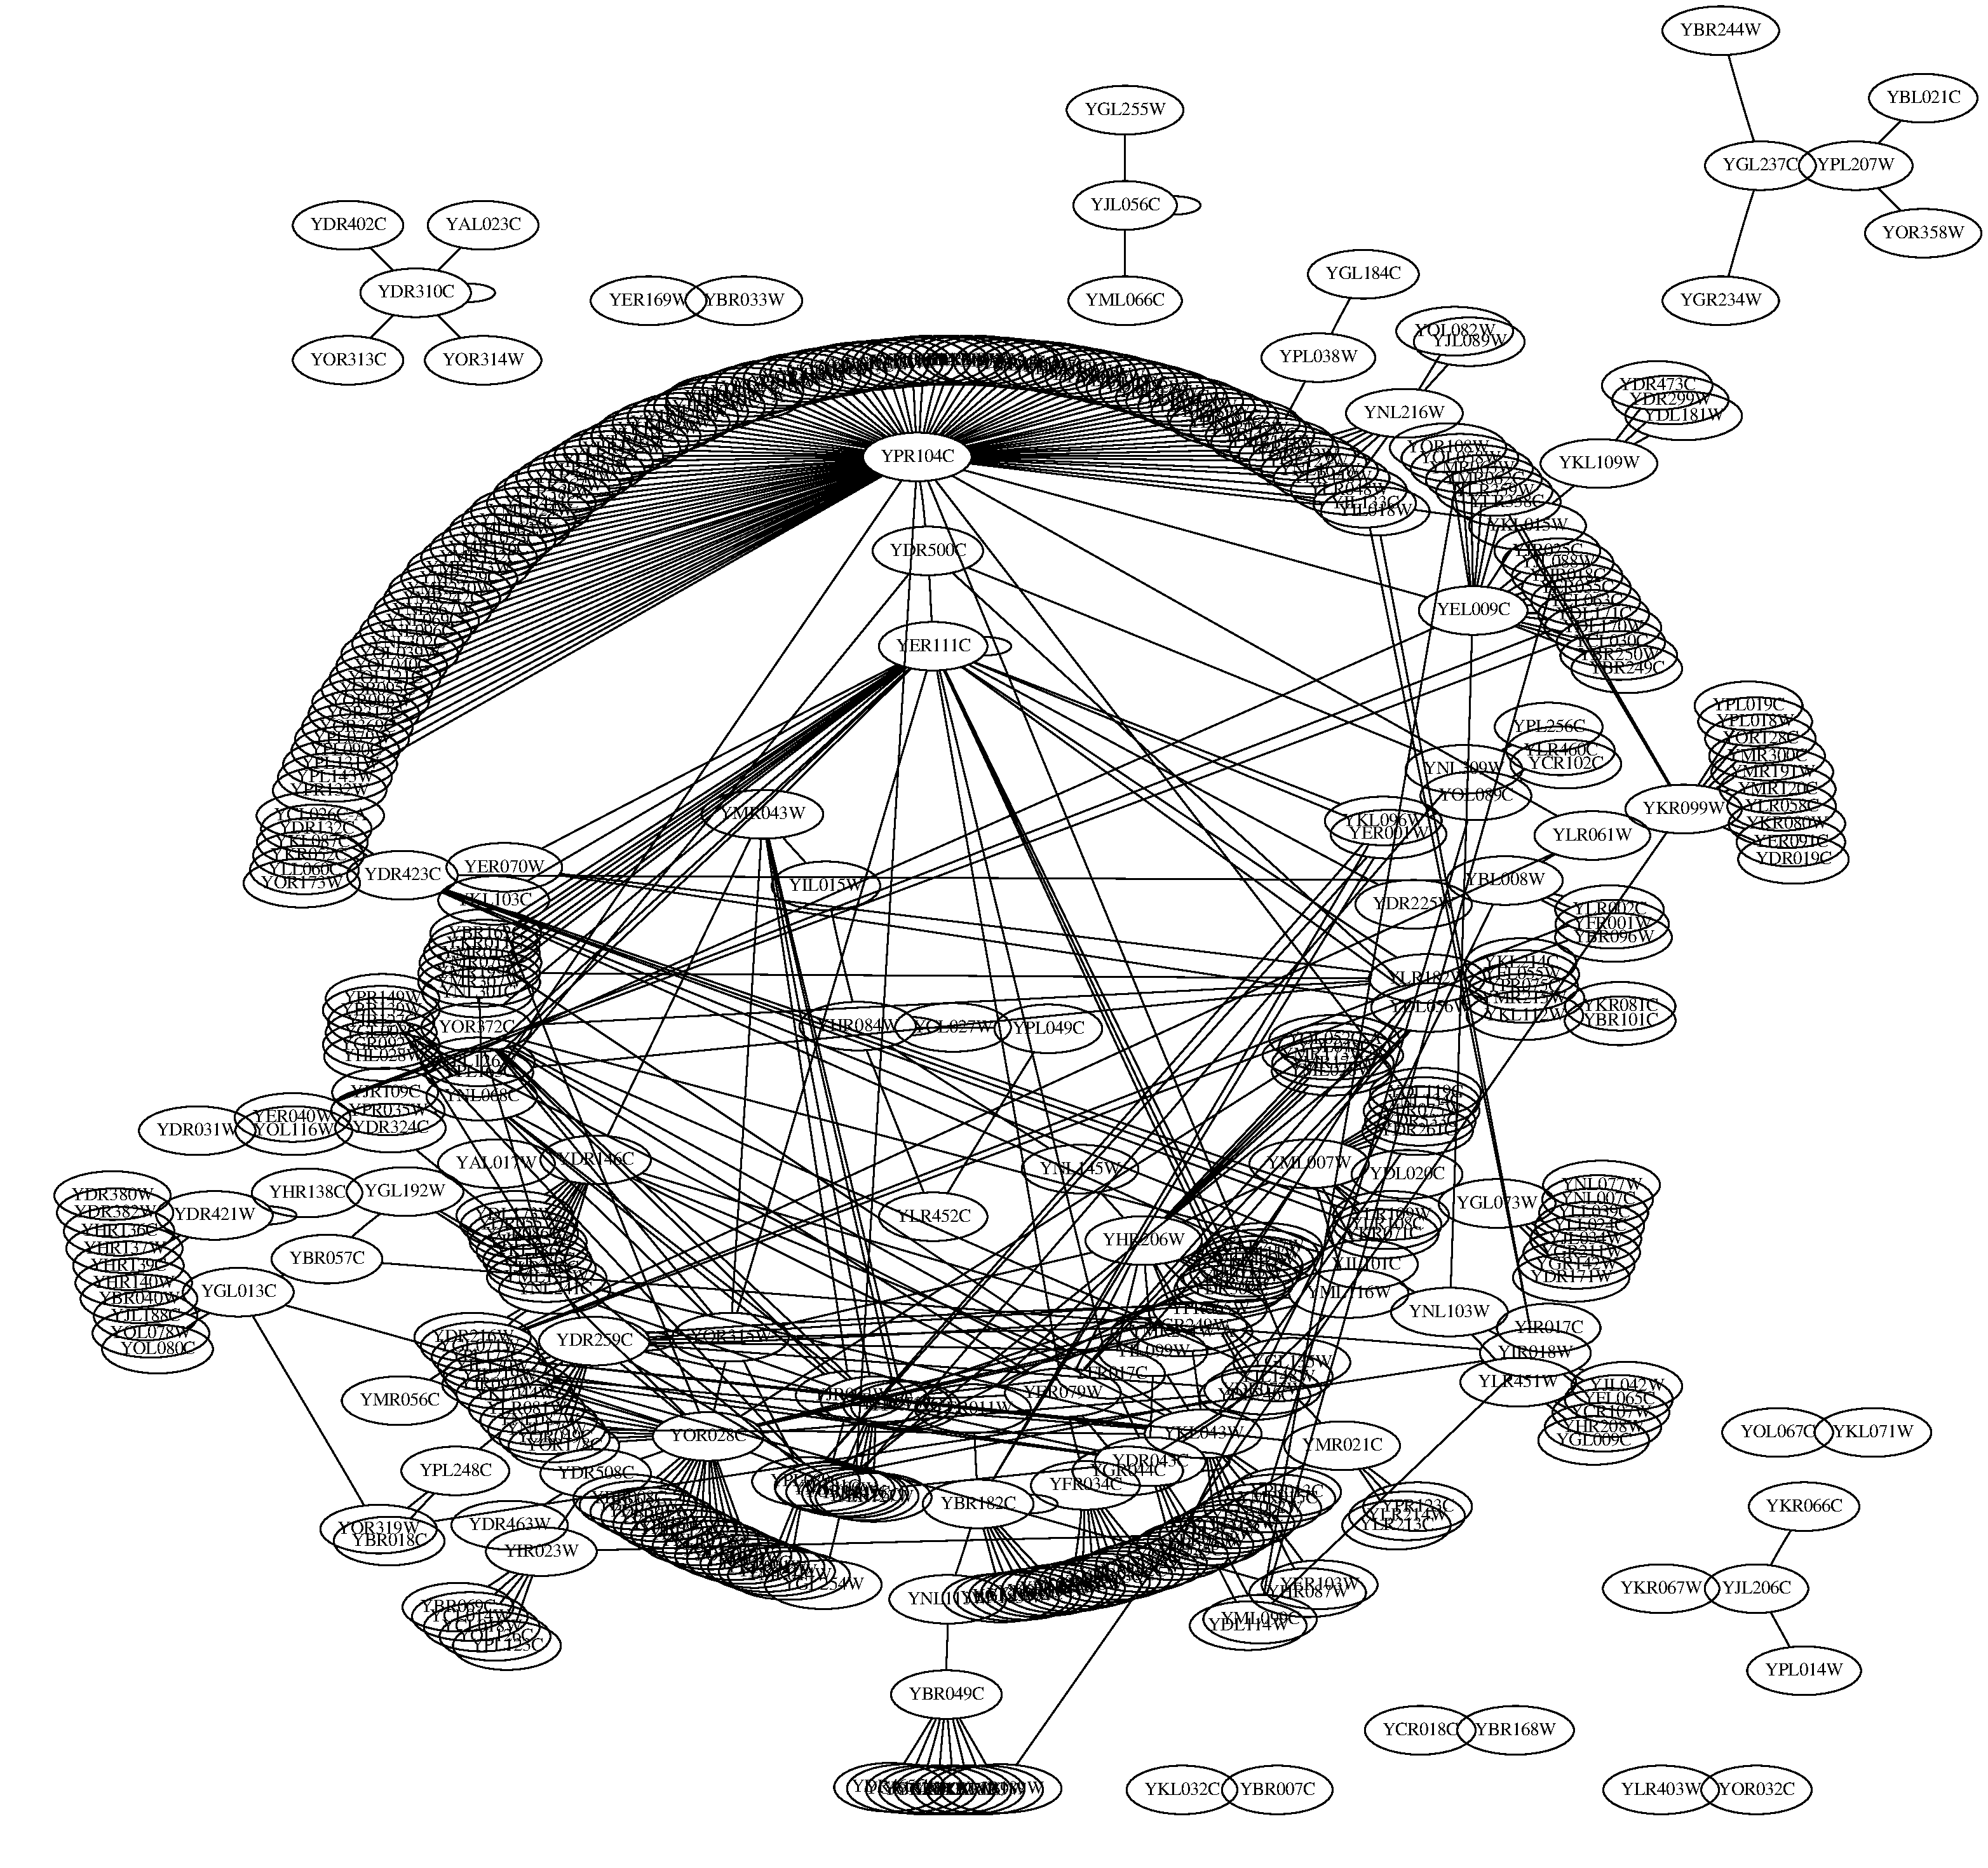
\includegraphics[scale=0.2]{chapter2/graph_0.0001.eps}}
   \subfigure[Constraints at p=0.001]{\label{fig:graph_constraints_0.001}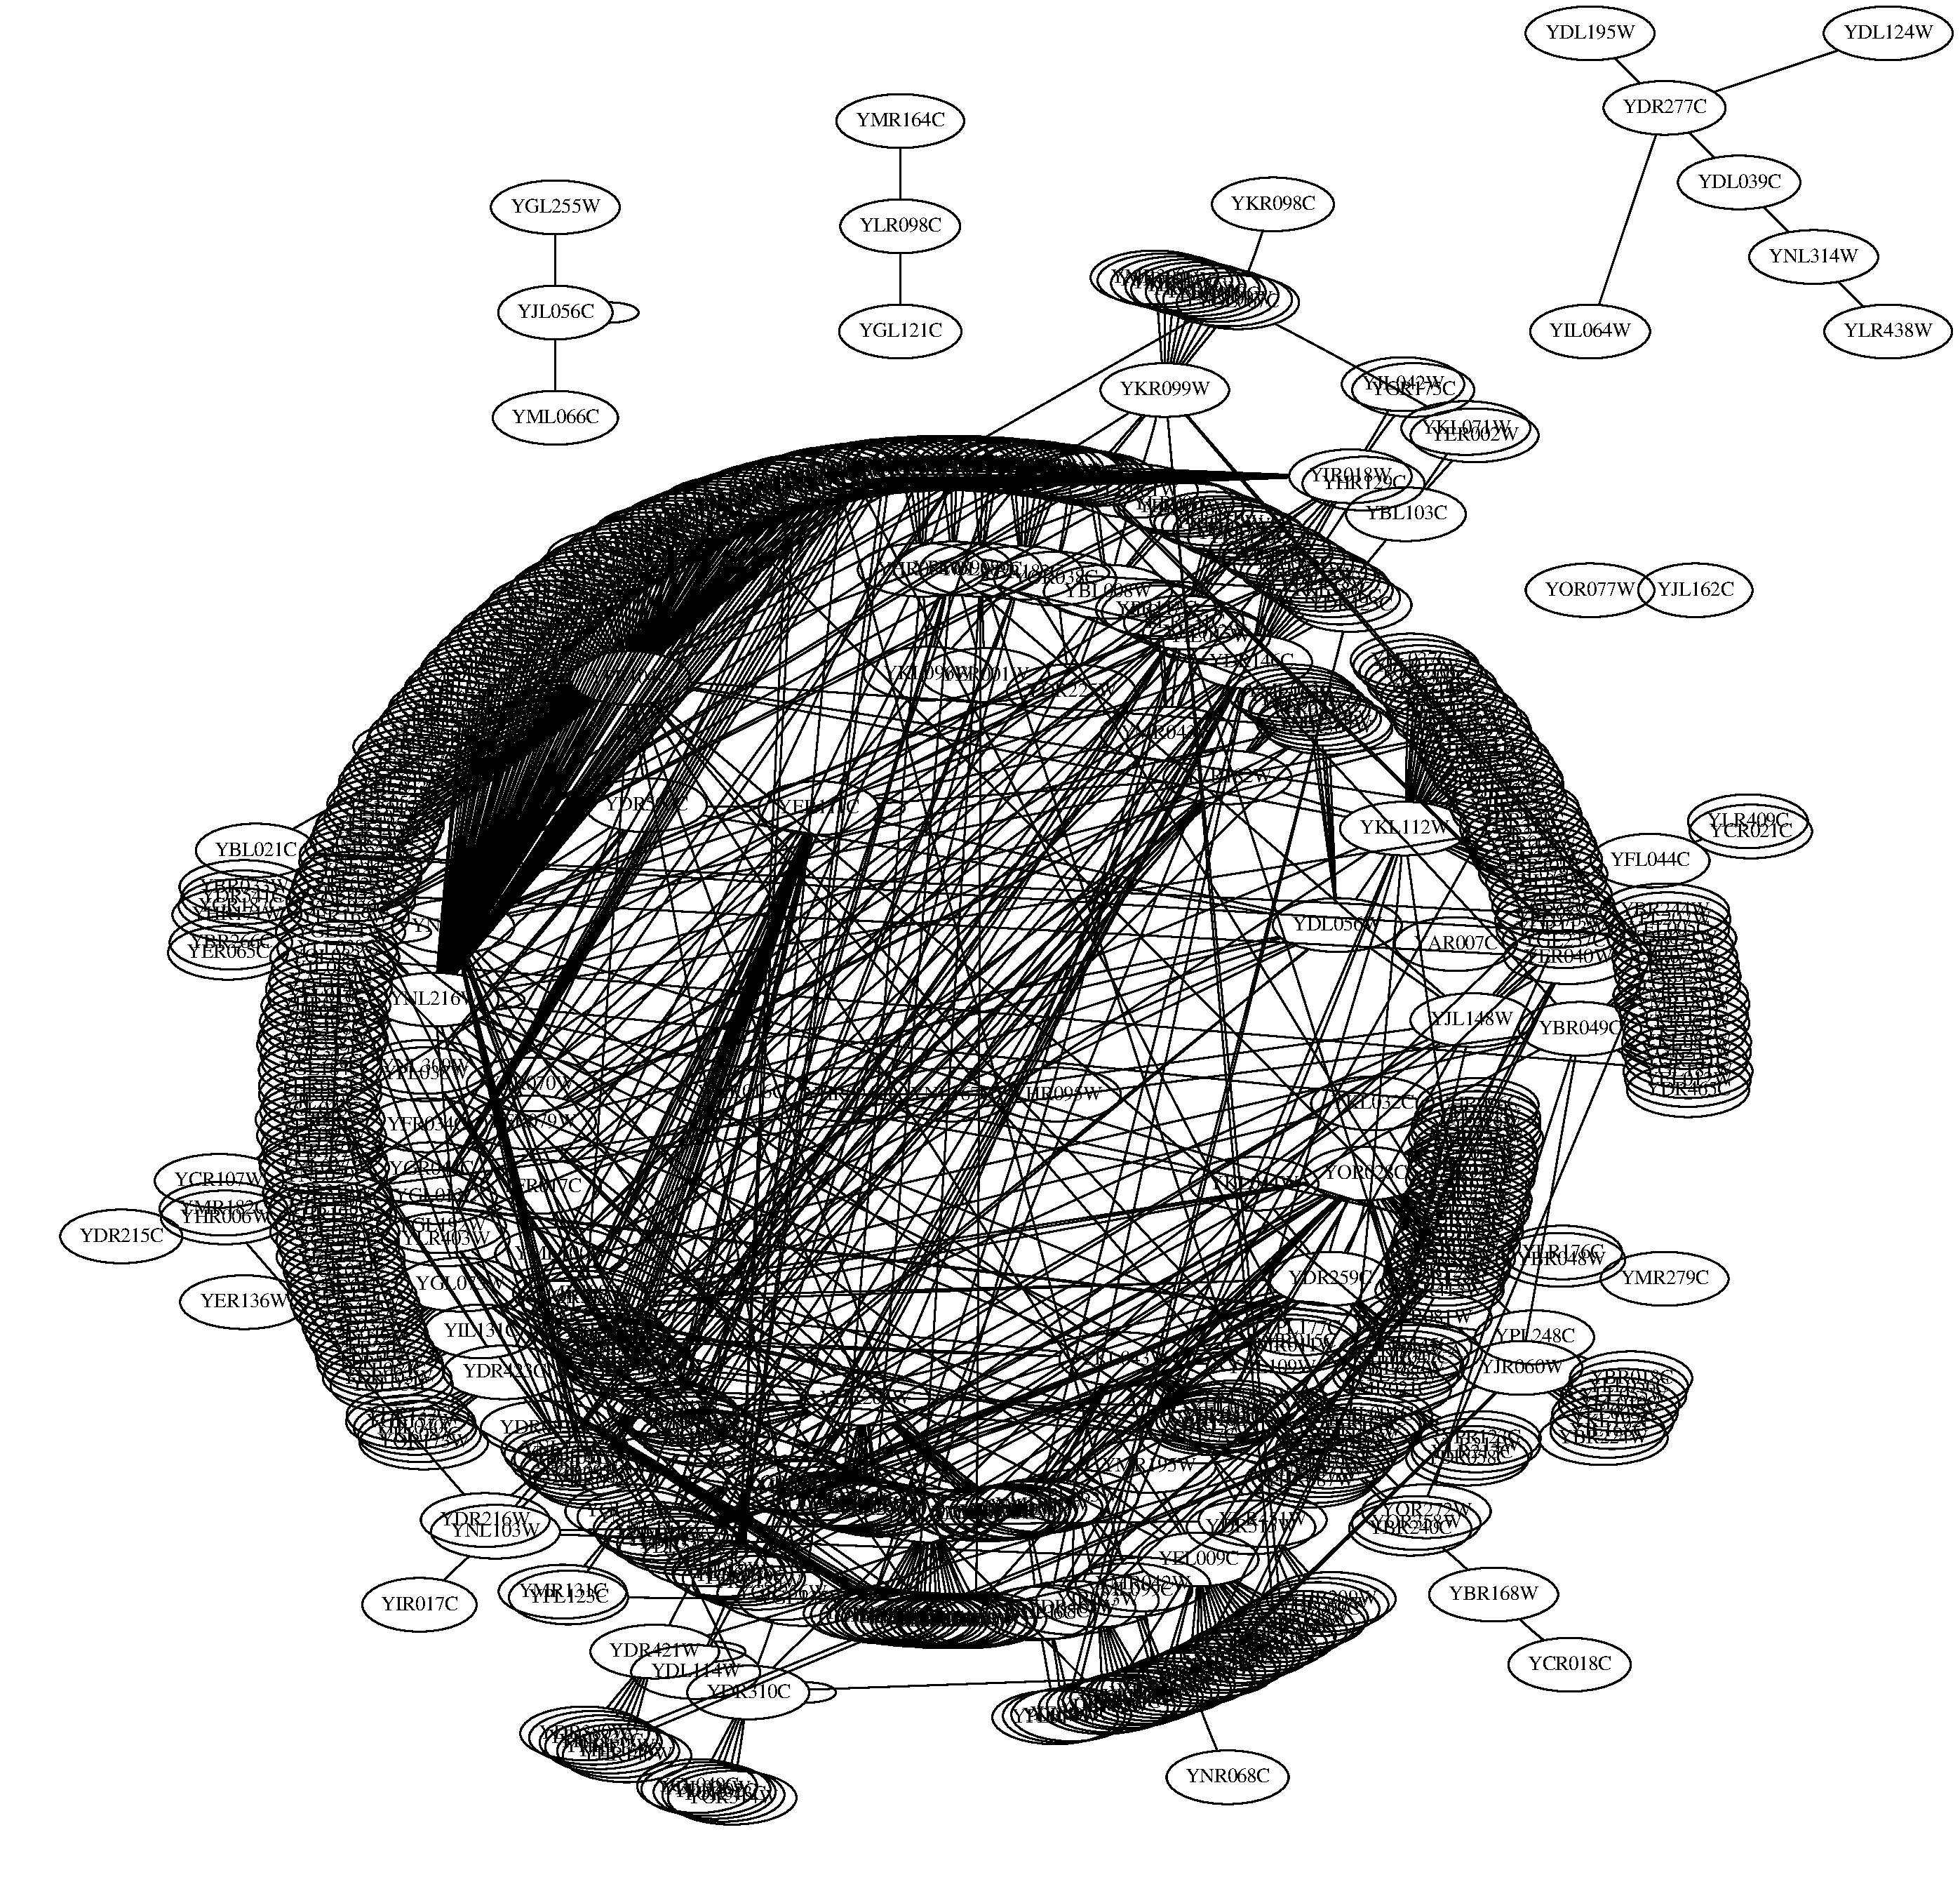
\includegraphics[scale=0.2]{chapter2/graph_0.001.eps}}

  \end{center}
\caption{Constraints derived from DNA-binding dataset at various p-value cutoffs}
\label{fig:constraints_with_pval}
\end{figure}

\begin{table}
\centering
\begin{tabular}{|c|c|c|c|}
\hline
p-value & \multicolumn{3}{|c|}{Number of Constraints} \\ \cline{2-4}
& All Genes & Common Genes (Stress) & Common Genes (Cell-cycle)\\
\hline
0.0001 & 2061  & 544   & 681\\
0.0005 & 3436  & 846   & 1032\\
0.001  & 4358  & 1053  & 1288\\
0.005  & 8562  & 1959  & 2442\\
0.01   & 12455 & 2776  & 3505\\
0.05   & 35917 & 7407  & 9713\\
0.1    & 63531 & 12579 & 17055\\
\hline 
\end{tabular}
\caption{Number of constraints from DNA-binding dataset at various p-value thresholds}
\label{tab:no_constraints}
\end{table}

\subsection{PPI dataset}
Another source of constraints is the popular PPI dataset from MIPS Comprehensive Yeast Genome Database (CYGD) \citep{Gueldener2006MPact}. It has been called a gold standard 
because of its quality and comprehensiveness \citep{yu2004annotation}. This dataset has information related to the proximity of proteins in yeast based on more than 
15446 protein-protein interaction records (9200 physical, 6400 genetic) which was compiled manually from the literature (3680 from single experiments) and published large-scale 
experiments. In addition to this, 268 manually extracted protein complexes as well as 783 complexes derived from large-scale experiments results in 87000 putative 
binary interactions. 

\subsection{TF-gene interactions dataset} \label{yeastract-db}
We also derived constrains from an independently curated database of known TF-gene interactions known as YEASTRACT(Yeast Search for Transcriptional Regulators And Consensus Tracking). 
YEASTRACT\footnote{interactions file created on 25/12/2008} \citep{Teixeira06yeastract} is a curated repository of 34471 regulatory associations between transcription factors and 
target genes in Saccharomyces cerevisiae, based on more than 1000 bibliographic references. In this database, the curators consider interaction to have occurred when there is change in the expression of the target gene owing to the deletion (or mutation) of the transcription factor-encoding gene. They also consider evidence based on TF binding to the promoter region of the target gene based on band-shift, footprinting or chromatin immunoprecipitation assays. They also describe potential associations but we have not considered them as we wanted to stick to known facts. 

\subsection{Semi-supervised spectral clustering} \label{sec:sssc}
We propose a semi supervised form of the spectral clustering method, which is detailed in Algorithm-\ref{alg:semi_sup_spectral_clustering} and shown in Figure-\ref{fig:semi_sup_spectral_clustering}. We are clustering microarray data, hence the genes can be considered the variables and their pairwise similarity values are calculated using a Gaussian affinity function. We have chosen this similarity function because it naturally encodes the local neighbourhood property and its value falls rapidly as the pairwise dissimilarity increases. Once we have this similarity matrix, we use the constraints derived from our secondary datasets to modify it. Since our constraints already encode our belief about potential interactions, we set each value in the similarity matrix to 1 (maximum similarity) if there is a 1 in the corresponding constraints matrix. All other values are left unchanged as we have no information regarding them. The idea behind changing the values to represent maximum similarity is to give the algorithm the maximum incentive to keep them in the same cluster. The resulting matrix is the final similarity matrix that we use for spectral clustering (Steps 3-7). We have used the algorithm suggested by \citet{ng2001onspectral}. The implementation was done in R using readily available libraries for linear algebra. 

We calculate the normalized Laplacian and then find its eigenvalues. If we believe there are $k$ clusters then eigenvectors corresponding to the $k$ smallest eigenvalues are chosen. If we arrange these $k$ eigenvectors column-wise then we end up with a $n \times k$ matrix. Each row of this matrix is then normalized to have unit norm. Then we cluster the rows using the k-means clustering algorithm. For all these integrated matrices, the k-means clustering of the eigenvectors was started from fixed centres. These 50 centres, each representing a cluster, were the genes encoding the TFs that had the highest numbers of DNA-interactions in the DNA-binding dataset. The idea behind this choice is to guide the clustering process to start from meaningful positions rather than random ones. Again, in step-4 of algorithm, we are proposing to take the eigenvectors corresponding to the largest k eigenvalues. This is because here we are using the Laplacian $L'$ instead of the form $L_{symmetric=}I-L'$ described earlier (refer eqn-\ref{eqn-lap_sym}). This changes the eigenvalues from $\lambda_{i}$ to $1-\lambda_{i}$. 

\begin{algorithm}
\caption{Semi-supervised spectral clustering}
\label{alg:semi_sup_spectral_clustering}
\begin{algorithmic}[1]
\REQUIRE Dataset ($X$), number of clusters ($k$) 

\STATE Calculate the symmetric similarity matrix $K_{n \times n}$  using Gaussian similarity function  $K_{ij}=exp \left( -\frac{{\parallel x_{i}-x_{j} \parallel}^{2}}{2\sigma^{2}}\right)$ if $i\neq j$, and set $K_{ii}=0$. 

\STATE Use the constraints to modify $K, K_{final}=K \oplus C$ where C is the constraints matrix. $K \oplus C$ implies that we set $K_{i,j}=1$ where $C_{i,j}=1$. 

\STATE Calculate the normalized Laplacian $L'=D^{-1/2}K_{final}D^{-1/2}$ where D is the diagonal matrix with $d_{jj}=\sum_{i}d_{ji}$ 

\STATE Find the eigenvectors $v^{1},v^{2},\dots,v^{k}$ corresponding to the largest k eigenvalues of $L'$. 

\STATE Use these k eigenvectors as columns to get $V_{n \times k}$. 

\STATE Normalize the rows to have unit norm, i.e., $U_{n \times k}$ such that $u_{ij}= v_{ij}/(\sum_{k}{v_{ik}^{2}})^{\frac{1}{2}}$

\STATE Cluster the points representing the rows of this matrix $(u_{i})_{i=1,...,n}$ using k-means algorithm into k clusters, $C_{1},C_{2},\dots,C_{k}$.  

\STATE Output clusters $A_{1},A_{2},\dots,A_{k}$ such that $A_{i}=\{x_{j}|u_{j}\in C_{i}\}$. This assigns the original point $x_{j}$ to cluster $A_{i}$ if $u_{j}$ is in cluster $C_{i}$. 

\end{algorithmic}
\end{algorithm}

\begin{figure*}[htp]
\centering
\scalebox{1.0}{
\begin{pspicture}(0,0)(16,12)
\psframe[framearc=0.1,linewidth=0.5mm](0,0)(16,12)

\rput(8.5,9.5){\Rnode{B}{$\begin{pmatrix}
1 & 1 & 0 & 0\\
0 & 0 & 0 & 1\\
1 & 0 & 1 & 1\\
0 & 0 & 0 & 0\\
\end{pmatrix}
$}}
\rput(5.1,9.5){\MyBox*[linecolor=lightgray]{4}{2}{Constraints Matrix derived from supervision sources}}

\pcline{->}(8.5,7)(8.5,5)
\pcline{->}(2.5,3.8)(3.5,3.8)

% microarray box and text
\rput(0.4,2.5){\Rnode{A}{\psgrid[gridwidth=0.02,subgridwidth=0.02,gridlabels=0.0pt,subgriddiv=4](0,0)(0,0)(2,3)}}
\rput(1.5,5.7){Conditions}
\rput(1.8,1.2){Microarray Data}
\rput{-270.0}(0.2,3.5){\rput(0,0){Genes}}

\rput(5.35,4){\Rnode{C}{$\begin{pmatrix}
0.2 & 0.5 & 0.6 & 0.2\\
0.3 & 0.3 & 0.3 & 0.3\\
0.2 & 0.4 & 0.6 & 0.2\\
0.7 & 0.4 & 0.3 & 0.6\\
\end{pmatrix}
$}}
\rput(5.5,1.2){Affinity Matrix}

\pcline{->}(7.6,3.8)(9.75,3.8)\nbput{\MyBox*[linecolor=lightgray]{3}{1}{set $A_{i,j}=1$ where $C_{i,j}=1$ }}
\rput(12,4){\Rnode{D}{$\begin{pmatrix}
1 & 1 & 0.6 & 0.2\\
0.3 & 0.3 & 0.3 & 1\\
1 & 0.4 & 1 & 1\\
0.7 & 0.4 & 0.3 & 0.6\\
\end{pmatrix}
$}}
\rput(12,1.2){Final Matrix}

\pcline{->}(14,3.8)(14.7,3.8)
\rput{-270.0}(15,3.8){\rput(0.1,-0.3){\MyBox*[linecolor=lightgray]{4}{1}{Spectral Clustering}}}

\end{pspicture} 
}

\caption{Semi-supervised spectral clustering}
\label{fig:semi_sup_spectral_clustering}
\end{figure*}

\subsection{Toy dataset explorations} \label{chap2:sec:spirals_dataset}
The semi-supervised problem can be stated as - there is a real distribution of data points that have certain pairwise similarities and an ideal clustering can be derived from it. 
We want to recover a clustering as close to the ideal one based on observing some noisy datasets and some facts (acting as constraints in our setup) that are known to us. Before we start work on real datasets 
we are going to show that semi-supervised clustering indeed is able to leverage external information in the form of pairwise constraints in order to better the clustering results. 

In order to do this, we take a toy dataset with non-linear patterns (points belonging to two classes are present in the form of two spirals) as seen in Figure-\ref{fig:spirals_original}. This data-set consists of two concentric clusters (300 points belonging to two classes) and was chosen because this is a specially 
hard problem on which many most traditional clustering algorithms fail. It also shows the effectiveness of spectral clustering in finding non-linear clusters which is not possible with 
traditional clustering algorithms. To represent the known facts or constraints, we extract some random constraints from it. Then to represent a noisy dataset, we skew the $\sigma$ with which pairwise similarities are computed from its optimum value to some random non-optimum value. After this, we study if the addition of progressively increasing quantities of the known relationships (constraints) improves the cluster quality of the noisy dataset.
We have used five-fold validation to study the effectiveness of our algorithm. So, in every run of the experiment 80\% of the data acts as training data 
while remaining 20\% is test data. The exact steps are detailed below 

\begin{enumerate}
 \item Take the spirals dataset which has two classes visually represented as red and black points as seen in Figure-\ref{fig:spirals_original}. 
We compute the optimal $\sigma$ with which to compute pairwise similarities by finding the least cumulative sum across all the clusters of sum of squared 
distance of all points in a cluster from its cluster centre as shown in Equation:\ref{maxent:eqn:withinss}. With this optimal $\sigma$ we compute the similarity matrix. 
We also generate a noisy version of it by changing the $\sigma$ to a random non-optimal value with which pairwise similarities are computed. 
The results of clustering with optimal and non-optimal $\sigma$ values are shown in Figures-\ref{fig:spirals_original} and \ref{fig:spirals_no_constraints} respectively.
 \item From the original dataset, we generate all possible pairs between all the points in each of the two classes respectively. Out of all these pairs, according to 5-fold cross validation procedure, take 4 parts as the training set and the remaining one as the testing set.
 \item Draw \textit{5} pairs of constraints from the training set randomly.
 \item Apply these pairwise constraints to the non-optimal similarity matrix, i.e., set the pairwise similarity of these data points to 1. Cluster it using spectral clustering.
 \item Compute the similarity between the resulting cluster and the original clustering using modified Rand's index (discussed in Chapter-3).
 \item Repeat this process 10 times by randomly drawing constraints from the training set.
 \item Increase the number of constraints used in Step-3 by 5 and repeat the whole process till perfect clustering is obtained all the time.
 \item Repeat this process 5 times for 5-fold cross validation.
 \end{enumerate}


\begin{figure}[p]
\centering
\subfigure[Original dataset clustering]{
\includegraphics[bb=0 0 720 720,scale=0.18]{images_only/semisup/spirals/100.eps}
\label{fig:spirals_original}
}
\subfigure[Noisy dataset clustering without any constraints]{
\includegraphics[bb=0 0 720 720,scale=0.18]{images_only/semisup/spirals/1.eps}
\label{fig:spirals_no_constraints}
}
\subfigure[Noisy dataset clustering with 5 constraints]{
\includegraphics[bb=0 0 720 720,scale=0.18]{images_only/semisup/spirals/5.eps}
\label{fig:spirals_5_constraints}
}
\subfigure[Noisy dataset clustering with 10 constraints]{
\includegraphics[bb=0 0 720 720,scale=0.18]{images_only/semisup/spirals/10.eps}
\label{fig:spirals_10_constraints}
}
\subfigure[Noisy dataset clustering with 15 constraints]{
\includegraphics[bb=0 0 720 720,scale=0.18]{images_only/semisup/spirals/15.eps}
\label{fig:spirals_15_constraints}
}
\subfigure[Noisy dataset clustering with 20 constraints]{
\includegraphics[bb=0 0 720 720,scale=0.18]{images_only/semisup/spirals/20.eps}
\label{fig:spirals_20_constraints}
}
\subfigure[Noisy dataset clustering with 25 constraints]{
\includegraphics[bb=0 0 720 720,scale=0.18]{images_only/semisup/spirals/25.eps}
\label{fig:spirals_25_constraints}
}
\subfigure[Noisy dataset clustering with 50 constraints]{
\includegraphics[bb=0 0 720 720,scale=0.18]{images_only/semisup/spirals/50.eps}
\label{fig:spirals_50_constraints}
}
\label{fig:spirals_visual}
\caption{Visual indication of Spirals dataset clustering quality improvement with increasing number of known constraints}
\end{figure}


\begin{figure}[p]
\centering
\subfigure[Run-1]{
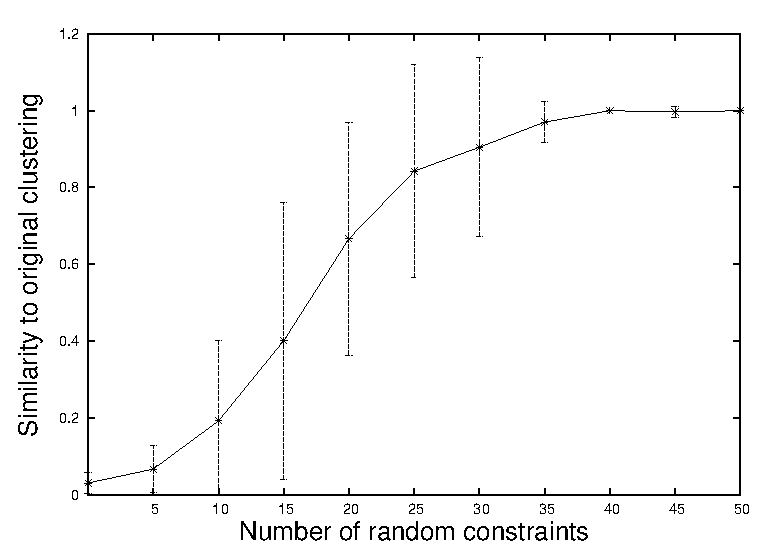
\includegraphics[bb=50 50 410 302,scale=0.5]{images_only/semisup/spirals/cv_fold1.eps}
\label{fig:spirals_cv_fold1}
}
\subfigure[Run-2]{
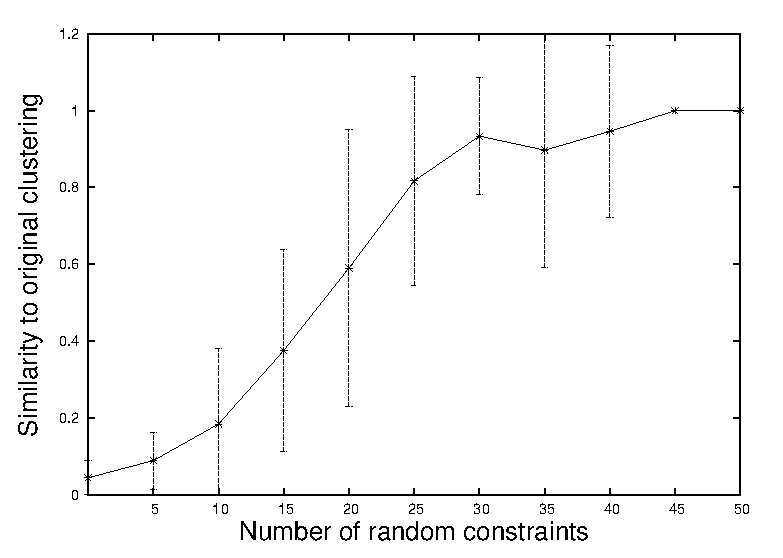
\includegraphics[bb=50 50 410 302,scale=0.5]{images_only/semisup/spirals/cv_fold2.eps}
\label{fig:spirals_cv_fold2}
}
\subfigure[Run-3]{
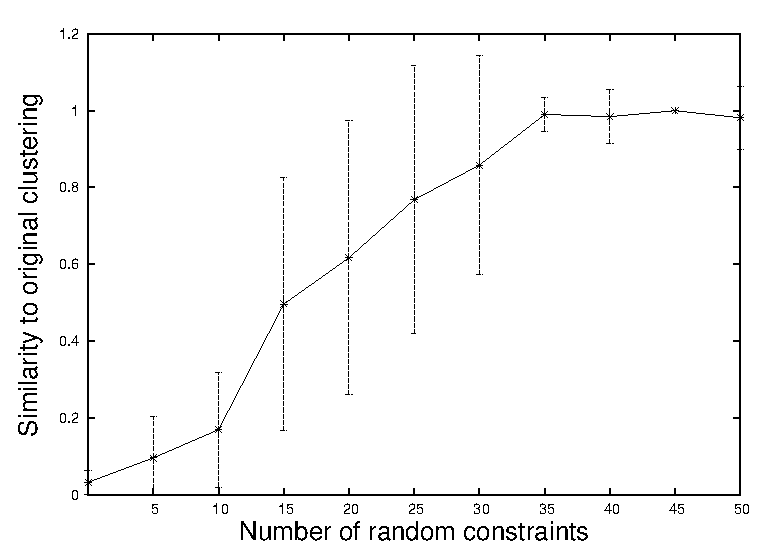
\includegraphics[bb=50 50 410 302,scale=0.5]{images_only/semisup/spirals/cv_fold3.eps}
\label{fig:spirals_cv_fold3}
}
\subfigure[Run-4]{
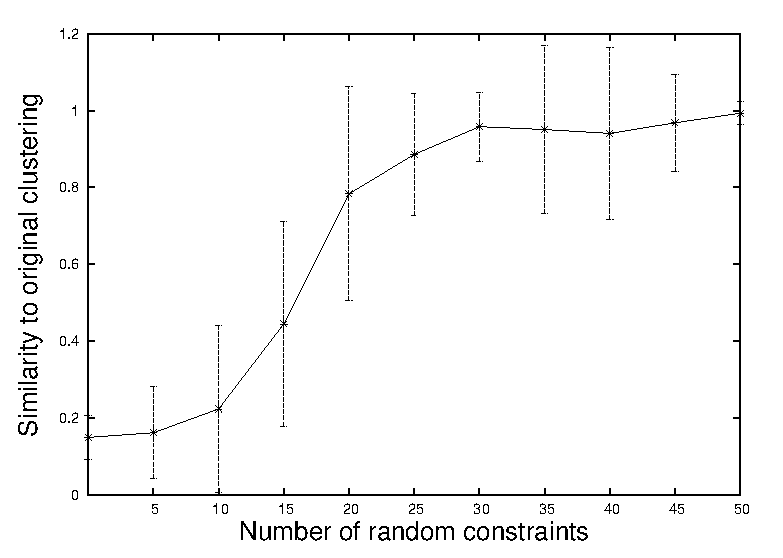
\includegraphics[bb=50 50 410 302,scale=0.5]{images_only/semisup/spirals/cv_fold4.eps}
\label{fig:spirals_cv_fold4}
}
\subfigure[Run-5]{
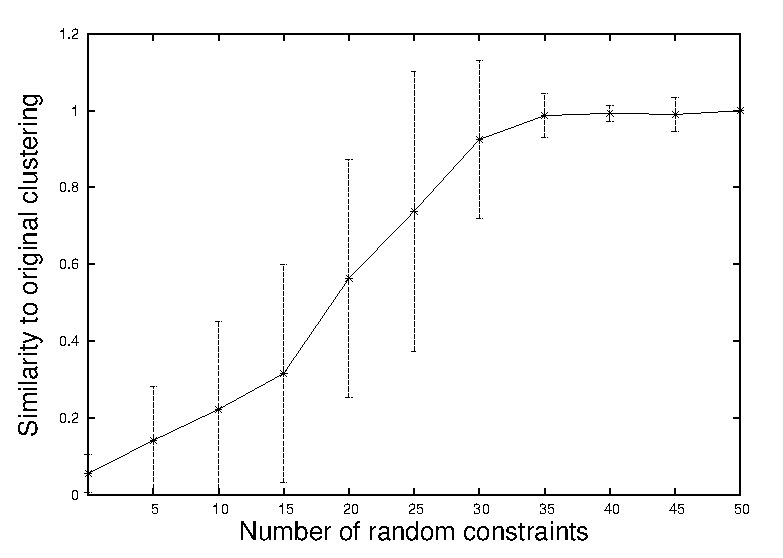
\includegraphics[bb=50 50 410 302,scale=0.5]{images_only/semisup/spirals/cv_fold5.eps}
\label{fig:spirals_cv_fold5}
}
\label{fig:spirals_cv}
\caption{Various runs showing clustering quality improvement with increasing number of known constraints}
\end{figure}

In Figure-\ref{fig:spirals_visual} we observe the results of one of the runs where increasing number of constraints are being applied. 
We see that the quality of clustering improves as the number of known constraints increase. We also observe that with a relatively small number of 
constraints ($50$), we are able to retrieve the original clustering.  

In Figure-\ref{fig:spirals_cv}, we see that in all the runs, clustering quality improves quickly as the number of known constraints are applied. 
The cluster similarity (to the original cluster) improves quickly with reducing standard deviation as the number of constraints increases. The goal of 
semi-supervised clustering is to use external knowledge in the form of known pairwise relations between variables in order to improve the quality of clustering. We have shown that applying more constraints indeed lead to better clustering.

\subsection{Parameter optimization} \label{chap2:sec:param_opt}
For any clustering algorithm, the most important decisions are the choice of the number of clusters and the free parameters. In our case, the similarity among gene pairs is calculated using a Gaussian similarity function and the only free parameter is the width of the Gaussian, $\sigma$. For any unsupervised task of an exploratory nature, the \textit{correct} number of clusters is data dependent. We chose to use 50 clusters in our experiments, based on earlier justifications by \citet{ihmels02revealing} and \citet{segal03module} which showed that the Saccharomyces Cerevisiae genome contains approximately 50 sets of functionally related genes. Both the authors have shown statistically that this number provides a better fit to the underlying data distribution, compared to a higher or lower numbers of modules.

In order to determine the value of $\sigma$, we chose to use cluster quality as the parameter to optimise in order to get the optimal value of $\sigma$. There are two major class of algorithms 
to validate the cluster quality. \textit{External} validation algorithms evaluate a clustering result based on the knowledge of the correct 
cluster class labels. This is external information that is not contained in the dataset, hence the name. This allows an objective evaluation and comparison of clustering algorithms based on known facts. In cases where no class labels are available, or the available labels are not reliable, 
we need to use \textit{internal} validation measures. Internal validation techniques do not use external class labels, but utilise information intrinsic to the data itself. They try to measure how well a given clustering corresponds to the natural cluster structure of the data.


\subsubsection{Internal Validation Indices} \label{chap2:subsec:cluster_validity_internal}
Internal measures take a clustering and the underlying dataset as the input, and use information intrinsic to the data to assess the quality of the clustering. 

\textit{Dunn's} index can be defined as 
\[
\text{Dunn's index}= \min_{C_{i}\in C} \left( \min_{C_{j} \in C \backslash i} \left( \frac{dist(C_{i},C_{j})}{\max_{C_{k}\in C}diam(C_{k})} \right) \right)
\]
where $diam(C_{k})$ is the maximum (complete) distance between two points within a cluster and $dist(C_{i},C_{j})$ is the minimum (single) distance between any two points in clusters $C_{i}$ and $C_{j}$. We can observe that the value of this index is high if the inter-cluster separation is high compared to the largest cluster diameter. This corresponds to a fundamental objective of good clustering, namely to maximize the inter-cluster separation and minimize the intra-cluster distances. Hence \textit{better} clustering will have \textit{higher} values of this index. This index, though very easy to comprehend, can be quite unstable especially in the presence of outliers. 

Another popular internal cluster quality validation index - \textit{Davies-Bouldin's} index that aims to identify sets of clusters that are compact and well separated, is defined as
\[
\text{Davies Bouldin's index}=\frac{1}{M} \sum_{i=1}^{M}\max_{\begin{subarray}{c}j=1\dots M \\ j\neq i \end{subarray}} \left( \frac{\sigma_{C_{i}}+\sigma_{C_{j}}}{\delta(C_{i},C_{j})} \right)
\]

where M is the total number of clusters, $\sigma_{C_{i}}$ is the average distance of all points in the $i_{th}$ cluster from the cluster centre and $\delta(C_{i},C_{j})$ is the distance between the cluster centres of the $i_{th}$ cluster and $j_{th}$ cluster. The value of this index decreases if clusters $i$ and $j$ are compact and their centres are far away from each other. Hence \textit{smaller} values of this index indicate better clustering.

The Silhouette index is another well known cluster validity index.
\[
s(i)=\frac{b(i)-a(i)}{max(a(i),b(i))} 
\]

For each datum $i$, let $a(i)$ be the average dissimilarity of $i$ with all other data within the same cluster. We can interpret $a(i)$ as how well matched $i$ is to the cluster it 
is assigned (the smaller the value, the better the matching). Then find the average dissimilarity of $i$ with the data of another single cluster. Repeat this for every cluster of 
which $i$ is not a member. Denote the lowest average dissimilarity to $i$ of any such cluster by $b(i)$. The cluster with this average dissimilarity is said to be the 
\textit{neighbouring cluster} of $i$ as it is, aside from the cluster $i$ is assigned, the cluster in which $i$ fits best.

From the above definition it is clear that
\[
-1<s(i)<1 
\]

For $s(i)$ to be close to 1 we require $a(i) \ll b(i)$. As $a(i)$ is a measure of how dissimilar $i$ is to its own cluster, a small value means it is well matched. 
A large $b(i)$ implies that $i$ is badly matched to its neighbouring cluster. Thus an $s(i)$ close to one means that the datum is appropriately clustered. If $s(i)$ is close to 
negative one, then by the same logic we see that $i$ would be more appropriate if it was clustered in its neighbouring cluster. The average $s(i)$ of a cluster is a measure of how tightly grouped all the 
data in the cluster are. Thus the average $s(i)$ of the entire dataset is a measure of how appropriately the data has been clustered. 

We chose to use Dunn's Index and Davies Bouldin's index in our studies to find the optimum value of $\sigma$.  The underlying logic of using this to choose $\sigma$ is to search for a value which results in the best quality clusters. 
We carried out this $\sigma$ optimization without using the supervision step, clustering only the microarray dataset because our objective is to study the impact of supervision. 
If we incorporate it prior to optimization then the constraints will impact the original similarity matrix.

We ran the spectral algorithm for a range of $\sigma$ values. The range of $\sigma$ values was determined as both the upper and lower extremes beyond which all the points 
resulted in a trivial clustering (single cluster).  For each $\sigma$ value, we did 10 runs as spectral clustering depends on k-means which has random starting points. 
We also repeated the k-means algorithm twenty five times, each run being initialised randomly, and chose the best clustering with the minimum total \textit{dispersion}. Dispersion was computed by taking the cumulative sum of within-cluster sum of squared distances (from each point to the centre) across all the clusters of a clustering run.  

\subsubsection{Stress dataset}

\begin{figure}[p]
 \centering
 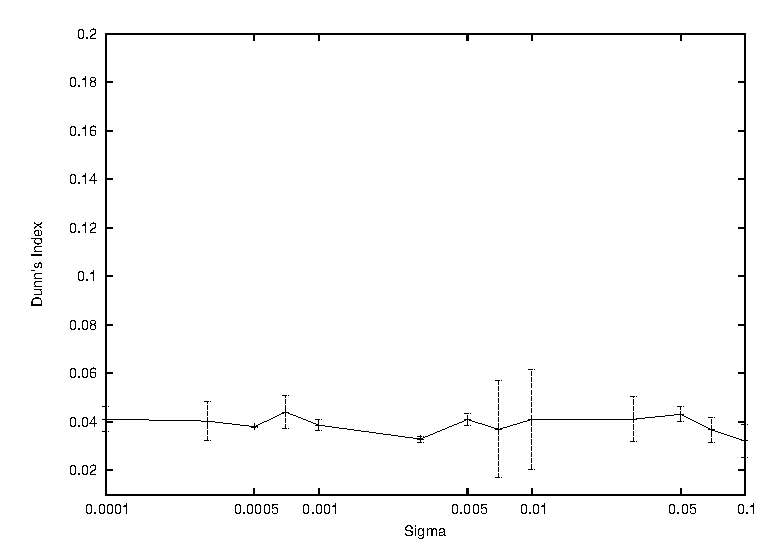
\includegraphics[scale=1.0]{images_only/semisup/results/plots/stress_dunn.eps}
 \caption{Stress dataset: Sigma optimization using Dunn's Index}
 \label{fig:stress_sigma_opt_dunn}
\end{figure}

\begin{figure}[p]
 \centering
 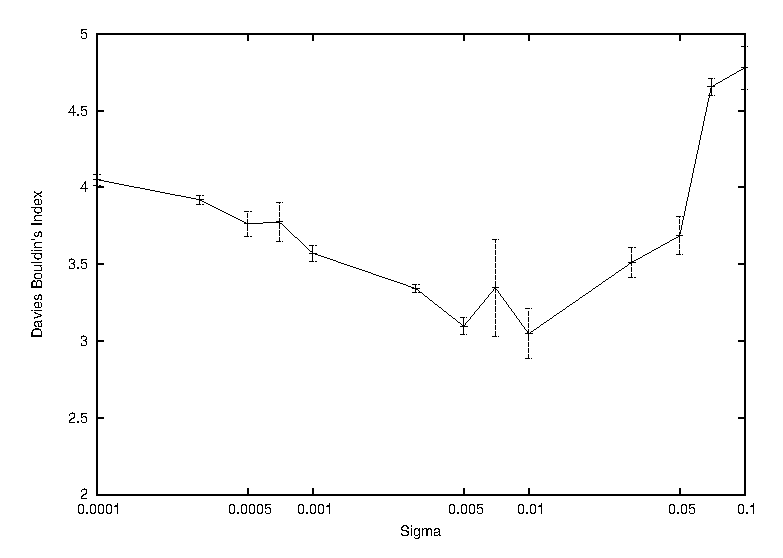
\includegraphics[scale=1.0]{images_only/semisup/results/plots/stress_davies.eps}
 \caption{Stress dataset: Sigma optimization using Davies Bouldin's Index}
 \label{fig:stress_sigma_opt_dav}
\end{figure}

The results for the Dunn's index based sigma optimisation for the stress dataset is shown in Figure-\ref{fig:stress_sigma_opt_dunn} which shows the mean values along with standard deviation error bars. 
The x-axis uses a log-scale because of the spread of the data.  For Dunn's index, where higher values are better, the plot has the optimal region between 0.003 and 0.005 where the 
standard deviations are low.
The maximum value (best clustering) at $\sigma=0.005$. It is worthwhile to note that the best quality clustering also has a very low standard deviation.

As seen in Figure-\ref{fig:stress_sigma_opt_dav}, the Davies-Bouldin's index, where lower values indicate better clustering, has its optimal region between 0.003 and 0.03. It has its minimum value (best clustering) at $\sigma=0.01$. However, the standard deviation is unacceptably high.
Considering that the next best value is $\sigma=0.005$ and it also has low standard deviation as well as it is in agreement with the Dunn's index values we choose this as the optimal sigma value for this dataset for further computations.  

\subsubsection{Cell-cycle dataset}

\begin{figure}[p]
 \centering
 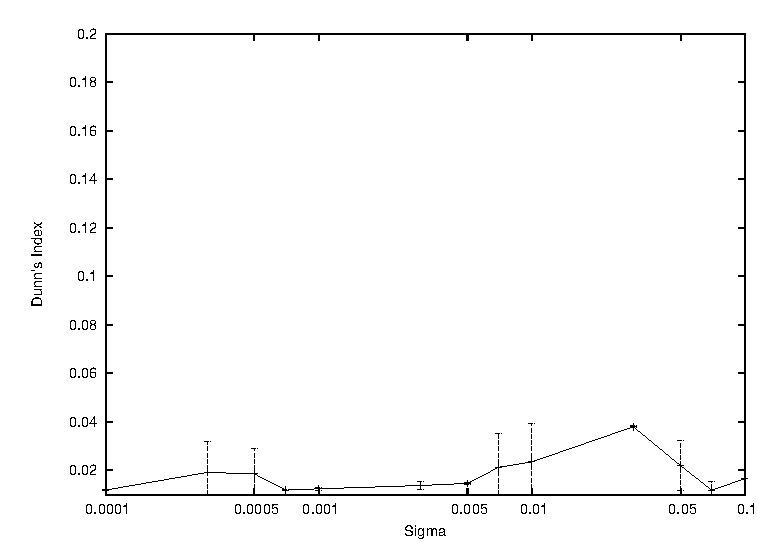
\includegraphics[scale=1.0]{images_only/semisup/results/plots/ccycle_dunn.eps}
 \caption{Cell-cycle dataset: Sigma optimization using Dunn's Index}
 \label{fig:ccycle_sigma_opt_dunn}
\end{figure}

\begin{figure}[p]
 \centering
 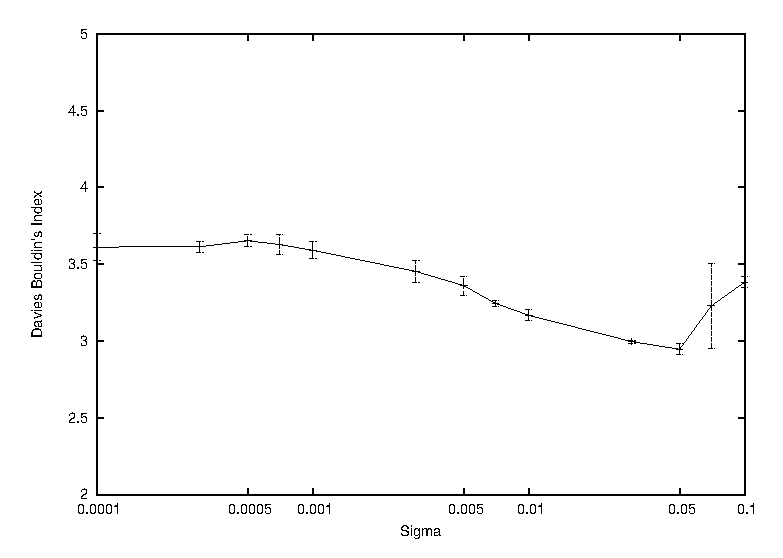
\includegraphics[scale=1.0]{images_only/semisup/results/plots/ccycle_davies.eps}
 \caption{Cell-cycle dataset: Sigma optimization using Davies Bouldin's Index}
 \label{fig:ccycle_sigma_opt_dav}
\end{figure}

The result for Dunn's index based optimisation for the cell-cycle dataset is shown in Figure-\ref{fig:ccycle_sigma_opt_dunn} which shows the mean values along with standard deviation error bars. 
The x-axis uses a log-scale because of the spread of the data.  Dunn's index has its maximum value (best clustering) at $\sigma=0.03$ and has a very low standard deviation there. 

As seen in Figure-\ref{fig:ccycle_sigma_opt_dav}, the Davies-Bouldin's index has its minimum value (best clustering) at $\sigma=0.05$ and the optimal region between 0.01 to 0.7. However, the standard deviation there is higher in comparison to at $\sigma=0.03$. 
Based on the consensus of both, we have used $\sigma=0.03$ value for all our further analysis for this dataset (cell-cycle). 

\begin{comment}
\section{Algorithm Validation}
After the parameter choices, we performed an independent validation of our results to check if the data integration was being effective. For this, we developed our own external cluster validity index, which is based on the concept of counting gene pairs within clusters that have a \textit{common} parent \ac{TF}.  We calculate a normalised count of such gene pairs in each cluster and use it as a measure of the biological significance of the cluster. The gene pairs with a common transcription factor were not derived from the DNA-binding dataset that we used for supervision but were taken from an independently curated database, YEASTRACT (refer Section-\ref{yeastract-db}). 

Suppose N is the total number of points in all the clusters, and K is the total number of clusters. If we define our clustering algorithm as an encoder, $k=E(i)$, which assigns each data point to a cluster $k$, then our Biological Significance Score, BSS is defined as

\[
BSS = \frac{1}{K}\sum_{i=1}^{K}\frac{1}{\binom{N_{i}}{2}}\sum_
{\substack{
a \neq b \\
E(a)=E(b)=i}}
 C((PTF(a) \cap PTF(b)) )
\]
where 
\begin{eqnarray*}
\binom{N_{i}}{2} & = & \frac{N_{i} * (N_{i}-1)}{2} \mbox{ ,}\\
N_{i} &=& \sum_{k=1}^{N}I(E(k)=i) \mbox{ and} \\
C(x) &=& \mbox{Cardinality of set x}\\
PTF(\textbf{g}) &=& \mbox{set of TFs that are known to bind to gene \textbf{g}}
\end{eqnarray*}

\begin{figure}[tp]
 \centering
 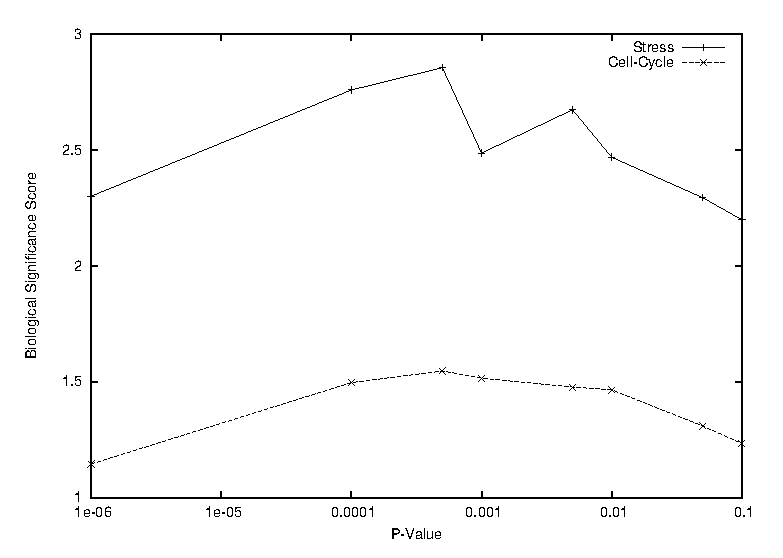
\includegraphics[scale=1.0]{chapter2/alg_valid.eps}
 \caption{Biological significance with constraints}
 \label{fig:bss_constraints}
\end{figure}

Using this (BSS) score, we were able to show that the algorithm can \textit{successfully use the information present in the DNA-binding data}. The original authors of the DNA-binding dataset \citep{harbison04transcriptional} have reported that they found the p-value of 0.001 to be the one which best represented known TF-DNA interactions. It maximizes inclusion of legitimate TFs and minimizes false positives. Lower values were too strict and higher values found many false positives. We were able to show a similar trend with our score (BSS) when different p-value cut-offs were used for selecting the constraints from the DNA-binding data. As discussed earlier in Section-\ref{chap2:sec:materials}, p-values are used as cutoffs in order to get our constraints. As a baseline, we also calculated the value when no constraints are applied (p-value=$10^{-6}$). 

From our results in Figure-\ref{fig:bss_constraints} for the stress dataset, we can see that with the addition of more constraints the cluster quality score improves till the p-value matches 0.0005 (which is very near the optimal p-value cut-off of 0.001 suggested by the original authors for best quality results for known TF-DNA interactions) and then gradually falls with increasing p-value after the peak. This signifies that when the number is larger than the optimum then the constraints represent noise and not-meaningful TF-gene interaction, and hence the clustering of microarray data is confused and the results get worse. From this result, we can conclude that the algorithm can meaningfully utilise the constraints. 

Now that we have seen that the algorithm really works and has been validated using an external index, we move on to study the biological significance of data integration. We would like to study if the resulting clusters are biologically any better or not when DNA-binding dataset constraints are used to guide the microarray data.
\end{comment}

\section{Statistical validation of results}
The datasets that we have, represent experiments done under particular conditions. If we base our results just on those datasets, the results that we obtain could be purely by chance because of the characteristics of those particular data-sets and it would be dangerous to draw conclusions based on those data-sets alone. 
Therefore, we have perturbed the datasets and report the mean and variance of results in order to justify that the results are not random. We begin by showing that spectral clustering results are immune to minor perturbations of data and the resulting clusters are not widely different from each other. The exact procedure is outlined as follows

\begin{enumerate}
  
\item We got the full stress and cell-cycle data-sets. The stress dataset had 6361 genes while cell-cycle dataset had 6353 genes including non-annotated open reading frames (NORFs). Since not much is known about the function of NORFs, we removed all the NORFs from the data-sets. 
That left us with 6251 genes in the stress data-set and 6257 genes in the cell-cycle data-sets. They had 156 and 60 experiment counts respectively.
 
\item We created ten perturbed data-sets from each of stress and cell-cycle datasets after sub-sampling (drawing 90\% of the genes randomly).

\item In order to compute the similarity matrix from the stress and cell-cycle datasets, we need to find the most optimum sigma. In order to do this we compute the Dunn's index and Davies Bouldin's index for each of the datasets. The same sigma is used for all the perturbed datasets because sigma should not change significantly for a data-set because of perturbation.

\item Once we have the sigma values, we cluster all the original and perturbed datasets and compute the Dunn's and Davies Bouldin's index for the resulting clusters. 
Then we report the mean and standard deviation of the indices. 
\end{enumerate}

\begin{table}
\centering
\begin{tabular}{|c|c|c|}
\hline
Serial No. & Dunn's index  & Davies Bouldin's index\\
\hline 
1 & 0.04398243 & 3.188676 \\
2 & 0.04306639 & 3.231177 \\
3 & 	0.04160664 & 3.136993 \\
4 & 	0.03673846 & 3.191647 \\
5 & 	0.04010983 & 3.154793 \\
6 & 	0.04787347 & 3.146264 \\
7 & 	0.02902327 & 3.212804 \\
8 & 	0.02349388 & 3.24161 \\
9 & 	0.03802108 & 3.163264 \\
10 & 	0.0563652 & 3.188100 \\
11 & 	0.03952356 & 3.168467 \\
\hline 
\end{tabular}
\caption{Dunn's and Davies Bouldin's index values for perturbed Stress dataset. The data indicates that the algorithm results in consistent cluster quality.}
\label{tab:stress_only_perturb}
\end{table}

\begin{table}
\centering
\begin{tabular}{|c|c|c|}
\hline
Serial No. & Dunn's index  & Davies Bouldin's index\\
\hline
1 & 0.03368041 & 2.989561 \\
2 & 0.04296991 & 3.026842 \\
3 & 0.01052886 & 3.127289 \\
4 & 0.03681052 & 2.967362 \\
5 & 0.04211076 & 3.005138 \\
6 & 0.01081028 & 3.112537 \\
7 & 0.03603748 & 3.027375 \\
8 & 0.02896914 & 2.975535 \\
9 & 0.03686515 & 3.038505 \\
10 & 0.03952675 & 2.871799 \\
11 & 0.02926203 & 3.00763 \\
\hline 
\end{tabular}
\caption{Dunn's and Davies Bouldin's index values for perturbed Cell-Cycle dataset. The data indicates that the algorithm results in consistent cluster quality.}
\label{tab:cellcycle_only_perturb}
\end{table}

\begin{table}
\centering
\begin{tabular}{|l|c|c|c|c|}
\hline
Description & \multicolumn{2}{|c|}{Dunn's index}  & \multicolumn{2}{|c|}{Davies Bouldin's index}\\
\hline
 & Mean & St. Dev & Mean & St. Dev\\
\hline
Stress only  & 0.0400 & 0.0087 & 3.1840 & 0.0341 \\
Cell cycle only & 0.0316 & 0.0113 & 3.0136 & 0.0693 \\
\hline 
\end{tabular}
\caption{Summary of mean and variance of individual datasets. This shows that our results are not random and a small perturbation in data doesn't change the results.}
\label{tab:stress_ccycle_perturb}
\end{table}

As we can see in the mean and standard deviation values in Table-\ref{tab:stress_ccycle_perturb}, the spectral clustering algorithm itself is quite stable with perturbations of 
data and resulting cluster qualities are not widely varying. We can see that the results of the cell cycle dataset have more variance in comparison to the stress dataset. 
This is seen in the results of both Dunn's and Davies Bouldin's indices.

Next we did a similar analysis of our proposed semi-supervised spectral clustering algorithm to demonstrate that it too does not produce results randomly and is consistent across 
sub-sampled datasets. In semi-supervised clustering, we are applying constraints in order to improve the quality 
of clustering. In order to justify that our results are not by accident, we need to sub-sample the data-sets as well as the constraints and then apply the sampled constraints. After this we need to compute the 
variance of cluster stability. We created ten constraints data-sets from each constraints dataset by sub-sampling (drawing 90\% of the genes randomly). Then we combined pairs of 
perturbed micro-array and constraints data-sets, cluster and then report the Dunn's and Davies Bouldin's clustering quality indices. We repeat this for all pairs. 
To reiterate, this was to demonstrate that our results are not random and that they are statistically valid.

\begin{table}[p]
\centering
\begin{tabular}{|c|c|c|}
\hline
Serial No. & Dunn's index  & Davies Bouldin's index\\
\hline
1 & 0.03089432 & 3.556163 \\
2 & 0.03321191 & 4.226998 \\
3 & 0.02888006 & 3.957121 \\
4 & 0.02731343 & 3.766975 \\
5 & 0.03100476 & 3.748136 \\
6 & 0.04172875 & 3.611934 \\
7 & 0.02727648 & 3.70486 \\
8 & 0.03053157 & 3.908451 \\
9 & 0.03172383 & 3.733790 \\
10 & 0.03420332 & 3.403322 \\
11 & 0.0312116 & 3.477314 \\
\hline 
\end{tabular}
\caption{Dunn's and Davies Bouldin's index values after combination of sub-sampled Stress and ChIP-chip datasets}
\label{tab:stress_chip_perturbed}
\end{table}


\begin{table}[p]
\centering
\begin{tabular}{|c|c|c|}
\hline
Serial No. & Dunn's index  & Davies Bouldin's index\\
\hline
1 & 0.04904669 & 3.563832 \\
2 & 0.05276492 & 3.552624 \\
3 & 0.03059342 & 3.65504 \\
4 & 0.03120301 & 3.729151 \\
5 & 0.03151477 & 3.712506 \\
6 & 0.03608802 & 3.581163 \\
7 & 0.02796911 & 3.691222 \\
8 & 0.04236918 & 3.713929 \\
9 & 0.03390614 & 3.513863 \\
10 & 0.0332141 & 3.770361 \\
11 & 0.03531316 & 3.625731 \\
\hline 
\end{tabular}
\caption{Dunn's and Davies Bouldin's index values after combination of sub-sampled Stress and PPI datasets}
\label{tab:stress_ppi_perturbed}
\end{table}

\begin{table}[p]
\centering
\begin{tabular}{|c|c|c|}
\hline
Serial No. & Dunn's index  & Davies Bouldin's index\\
\hline
1 &  0.02777897 & 3.523816 \\
2 & 0.01287181 & 3.365275 \\
3 & 0.03601802 & 3.40098 \\
4 & 0.02776162 & 3.563739 \\
5 & 0.03599602 & 3.4396 \\
6 & 0.03671904 &  3.631468 \\
7 &  0.03603748 & 3.429060 \\
8 &  0.03518232 & 3.406876 \\
9 &  0.03876811 & 3.441273 \\
10 &  0.03532557 & 3.563856 \\
11 &  0.03534912 &  3.297843 \\
\hline 
\end{tabular}
\caption{Dunn's and Davies Bouldin's index values after combination of sub-sampled Cell-cycle and ChIP-chip datasets}
\label{tab:ccycle_chip_perturbed}
\end{table}

\begin{table}[p]
\centering
\begin{tabular}{|c|c|c|}
\hline
Serial No. & Dunn's index  & Davies Bouldin's index\\
\hline
1 & 0.01359537 & 3.289819 \\
2 & 0.04214127 & 3.544937 \\
3 & 0.02760288 & 3.562716 \\
4 & 0.03359021 & 3.419286 \\
5 & 0.03575436 & 3.438057 \\
6 & 0.03155372 & 3.764982 \\
7 & 0.03372035 & 3.576627 \\
8 & 0.02835823 & 3.557268 \\
9 & 0.03526276 & 3.68283 \\
10 & 0.04028695 & 3.344107 \\
11 & 0.03255372 & 3.578498 \\
\hline 
\end{tabular}
\caption{Dunn's and Davies Bouldin's index values after combination of sub-sampled Cell-cycle and PPI datasets}
\label{tab:ccycle_ppi_perturbed}
\end{table}

\begin{table}[p]
\centering
\begin{tabular}{|c|c|c|}
\hline
Serial No. & Dunn's index  & Davies Bouldin's index\\
\hline
1 & 0.02746167 & 4.34282 \\
2 & 0.03222197 & 4.390683 \\
3 & 0.02823931 &  4.232013 \\
4 & 0.02939493 &  4.362611 \\
5 & 0.02742154 & 4.269306 \\
6 & 0.02760314 & 4.416886 \\
7 & 0.02787649 & 4.089062 \\
8 & 0.02709607 & 3.842911 \\
9 & 0.02733636 & 4.4379 \\
10 & 0.02829065 & 4.429637 \\
11 & 0.02746646 &  4.165664 \\
\hline 
\end{tabular}
\caption{Dunn's and Davies Bouldin's index values after combination of sub-sampled Cell-cycle and Yeastract datasets}
\label{tab:ccycle_yt_perturbed}
\end{table}

\begin{table}
\centering
\begin{tabular}{|l|c|c|c|c|}
\hline
Description & \multicolumn{2}{|c|}{Dunn's index}  & \multicolumn{2}{|c|}{Davies Bouldin's index}\\
\hline
 & Mean & St. Dev & Mean & St. Dev\\
\hline
Stress-Chip & 0.0316 & 0.0040 & 3.7359 & 0.2339 \\
Stress-PPI & 0.0324 & 0.0071 & 3.6367 & 0.0431 \\
Stress-YT & 0.0367 & 0.0080 & 3.6463 & 0.0843 \\

\hline
Cell-cycle-Chip & 0.0325 & 0.0074 & 3.4603 & 0.0992 \\
Cell-cycle-PPI & 0.0322 & 0.0076 & 3.5236 & 0.1406 \\
Cell-cycle-YT & 0.0282 & 0.0015 & 4.2709 & 0.1820 \\
\hline 
\end{tabular}
\caption{Mean and variance of all combined datasets. This shows that the results of semi-supervised clustering are not random and small perturbations in data do not change the results wildly.}
\label{tab:mean_stdev_combined_perturbed}
\end{table}

Tables-\ref{tab:stress_chip_perturbed} to \ref{tab:ccycle_yt_perturbed} show the cluster quality results of individual combinations of datasets. We have compiled the mean 
and standard deviation values of these individual results in Table-\ref{tab:mean_stdev_combined_perturbed}. 

We observe that the results of semi-supervised clustering are stable with perturbations in both the datasets. For the stress dataset the variability in results is even lower than
 observed for the stress only dataset according to Dunn's index. But the Davies Bouldin's index displays higher variability. For the cell-cycle dataset, the variability according to Dunn's
 index has fallen in all the instances of integration as compared to the cell-cycle only dataset. However, again Davies Bouldin's index is displaying higher variability.
  
Now that we are confident of clustering quality as well as the semi-supervised clustering results, 
we analyse the biological significance of combinations. For this, we need to observe the results of combinations of original datasets 
and not the perturbed versions. 

\section{Biological Significance Analysis}
Evaluation of the results of our clustering algorithm requires careful consideration since there are no gold standards against which performance can be measured. 
The two prominent types of cluster validation measures are \textit{internal} and \textit{external} validation indices. As indicated earlier, internal indices take a dataset and 
the resulting clustering and use information fully intrinsic to the data itself to assess the quality of clustering while external validation indices use information independent 
of the dataset for validating the clustering. We already saw the use of an internal validity measure for parameter ($\sigma$) selection. As they are fully dependent on the 
data itself, internal indices do not give any indication of the biological significance of the resulting clusters.  

There are various other methods that have been used in the past for external validation, many of which have used the information available in the Gene Ontology. 
They calculate the statistical significance of the gene ontology terms in the clusters. While this method gives us general ideas about which clusters might represent 
what functions, it doesn't allow us to functionally compare different clustering results \textit{numerically}. Some attempts have been made to provide 
such a numerical index using mutual information and related concepts by \citet{Gibons2002Judging} and \citet{gatviks03scoring} using Gene Ontology annotations. 

In order to compare two sets of clusters, e.g. before and after data integration, we have used the technique suggested by \citet{Gibons2002Judging}. We briefly discuss 
the ideas of these two papers and then justify our rationale behind our choice.

\subsection{Numerical Biological Significance comparison (using mutual information)} \label{semisup:num_biosig_mi}
\citet{Gibons2002Judging} devised a figure of merit, z-score, based on mutual information between a clustering result and gene annotation data. The z-score indicates relationships between 
clustering and annotation, relative to a clustering method that randomly assigns genes to clusters. A higher z-score indicates a clustering result that is further 
from random. 

The GO  project is a collaborative effort to address the need for consistent descriptions of gene products in different databases. The GO collaborators are developing three structured, controlled vocabularies (ontologies) that describe gene products in terms of their associated biological processes (BP), 
cellular components (CC) and molecular functions (MF) in a species-independent manner. The project not only writes 
and maintains the ontologies themselves but more importantly also makes cross-links between the ontologies and the genes and gene products in the collaborating databases. 
It is organized as three separate tree structured sets (directed acyclic graph (DAG)), consisting of directed edges and vertices, such that each vertex may be 
descended from several others. Annotation of a gene with a descendant attribute implies that the 
gene holds all ancestor attributes. They have parsed annotation from SGD of S. cerevisiae genes with GO attributes in such a way that attributes are inherited 
through the hierarchy, producing a table of \string~6300 genes and \string~2000 attributes in which a 1 in position (i,j) indicates that the gene i is known to possess attribute 
j, and a 0 indicates our lack of knowledge about whether gene i possesses attribute j. In other words, absence of annotation is not the same as absence of function.

We have not used the graphical structure and inter-relationships among the terms in the ontology graph. We have used only the relationship maintained between the 
ontology and genes and gene products across the BP category of it as we were interested in ascertaining whether the cluster were enriched in certain biological processes.

With this gene-attribute table, they construct a contingency table for each cluster-attribute pair, from which they compute the entropies for each cluster-attribute pair ($H_{A_{i}C}$), 
for the clustering result independent of attributes ($H_{C}$), and also for each of the $N_{A}$ attributes in the table independent of clusters ($H_{A_{i}}$). 
Using the definition of mutual information between two variables X and Y, $MI(X,Y) \equiv H(X)+H(Y)−H(X,Y)$, and assuming both absolute and conditional independence of attributes, 
they expand the total mutual information as a sum of mutual information between clusters and each individual attribute. 
They compute the total mutual information between the cluster result C and all the attributes $A_{i}$ as:
\[
MI(C,A_{1}A_{2},....A_{N_{A}}) = \sum_{i}MI(C,A_{i}) = N_{A}H_{C} + \sum_{i}H_{A_{i}}-\sum_{i}H_{A_{i}}C
\]

where summation is over all attributes i.

They score a partitioning as follows: 
\begin{itemize}
 \item Compute MI for the clustered data ($MI_{real}$), using the attribute database derived from GO/SGD; 
 \item Compute MI again, for a clustering obtained by randomly assigning genes to clusters of uniform size ($MI_{random}$), repeating until a distribution of values is obtained; 
 \item Compute a z-score for $MI_{real}$ and the distribution of $MI_{random}$ values (with mean $m_{random}$ and standard deviation $s_{random}$) according to 
\[
z = \frac{MI_{real}-m_{random}}{s_{random}} 
\]
\end{itemize}

The z-score can then be interpreted as a standardized distance between the MI value obtained by clustering and those MI values obtained by random assignment of genes to clusters. 
The larger the z-score, the greater the distance, and higher scores indicate clustering results more significantly related to gene function.

Clusters to which genes were randomly assigned were chosen to be as nearly uniform in size as possible, so that some of the success of a clustering algorithm relative 
to random may derive from producing nonuniform cluster size distributions. Uniform cluster sizes yield the highest value of $H_{C}$, which allows for the highest 
possible $MI(C,X)$ for some variable $X$ of unknown entropy $H(X)$, because $0 \leq MI(C,X) \leq min(H_{C},H(X))$.

\citet{gatviks03scoring} devised a method that is based on projecting vectors of biological attributes of the clustered elements onto the real line, such that the ratio 
of between-groups and within-group variance estimators is maximized. The projected data are then scored using a non-parametric analysis of variance test, and the 
score's confidence is evaluated.

Even though both the techniques use non-parametric techniques, we chose the former because \citet{gatviks03scoring} have indicated that their technique is sensitive to small perturbations in 
the clustering solution.  


\subsubsection{Results}
\begin{table}
\centering
\begin{tabular}{|l|l|l|l|}
\hline
Description & Before integration & After integration & \% Gain\\
\hline
Stress with ChIP-chip dataset & 89.2 & 86.7 & -2.8\\
Stress with PPI dataset & 89.2 & 95.2 & 6.72\\
Stress with Yeastract dataset & 89.2 & 93.2 & 4.48\\
\hline
Cell-cycle with ChIP-chip dataset & 52.2 & 44.8 & -14.17\\
Cell-cycle with PPI dataset & 52.2 & 55.2 & 5.74\\
Cell-cycle with Yeastract dataset & 52.2 & 64.8 & 24.13\\
\hline 
\end{tabular}
\caption{Biological Significance before and after semi-supervised integration}
\label{tab:biol_significance}
\end{table}

We started with the full set of stress and cell-cycle datasets as discussed earlier. The reason we had chosen stress and cell-cycle datasets is because they represent two ends of the spectrum \citep{amos05integrative}. 
For the ChIP-chip, PPI and Yeastract datasets, we took all the interactions that were between the common set of genes between the microarray and the interactions datasets. 
The biological significance index values before and after semi-supervised clustering are in Table-\ref{tab:biol_significance}. 

The different initial biological significance values for stress and cell-cycle datasets (89.2 and 52.2 respectively) are because of the nature of the data. Stress on the organism 
leads to extremely high levels of activity 
in the expression levels and many more genes are coordinating together which leads to higher significance values. Cell-cycle on the other hand is a routine activity and the 
expression patterns of genes do not change so extremely leading to smaller significance values.

We observe that the stress dataset when combined with ChIP-chip constraints leads to 
slightly worse biological significance (-2.8\%) after the combination. On the other hand, combination with PPI and Yeastract constraints lead to better significance values (6.72\% and 4.48\% respectively). For 
the cell-cycle dataset too, combination with ChIP-chip dataset leads to reduced biological significance (-14.17\%). When combined with both PPI and Yeastract constraints the biological significance 
has gone up. Based on the results we could say that the ChIP-chip dataset is probably the noisiest and does not bring much new information leading to reduced significance for the original datasets. 
One of the reasons for this is that integration could be meaningful if each of the datasets complement the other. If there are 
a lot of conflicting information in each of the datasets then the resulting matrix will have a lot of noise and this will be reflected in the final clusters. We know that ChIP-chip and PPI are uncurated datasets i.e. the information there is derived from experiments which always has the possibility of inducing noise. On the other hand Yeastract 
dataset is a manually curated dataset. That is the reason we see a high improvement when combined with it for both stress and cell-cycle datasets. 
  
The goal of integration is to have more biologically relevant clusters from which hypotheses could be derived to be carried out and validated in wet labs. All our result data is available upon request. 

\subsection{Qualitative Biological Significance (using Gene Ontology annotations)} \label{semisup_biosig_go}
Now that we have results of quantitative biological significance before and after applying our algorithm, we would also like to qualitatively analyze the resulting clusters after 
applying our algorithm. We would like to identify the biological processes represented by the genes in each cluster. For this, we use Genomica's gene set enrichment module available online (\url{http://genie.weizmann.ac.il/genomica_web/enrichment/gene_sets.jsp}). It allows us to compute 
p-value of a \textit{HyperGeometric} distribution to find the enrichment of individual genes in a cluster as detailed below.

The result of a clustering algorithm is a set of gene clusters. In order to find out how biologically significant the cluster set is, we have again used 
Gene Ontology \citep{GO} annotations. So, from this database, we extract annotations for each gene in a cluster. Then, we would like to know if any GO term is  overrepresented in the cluster 
compared to that happening by chance. This can be answered by \textit{p-value} from statistical hypothesis testing. 
The p-value is the probability of obtaining a result at least as extreme as the one that was actually observed, given that the null hypothesis is true. 
So, under our null hypothesis that the set of genes is randomly picked from the whole gene population we compute this p-value using a \textit{HyperGeometric} distribution 
as the probability that $n$ randomly chosen genes will have $k$ or more annotations of a certain type and can be written as

\[
P(X \geq k) = \sum_{i=k}^{n} \frac{\binom{K}{i} \binom{N-K}{n-i}}{\binom {N}{n}}
\]
 
Here, the total number of genes is $N$ of which $K$ are known to be of the particular annotation type that we are interested in. The cluster that we test for over-representation has $n$ genes.

In all our computations, we have only used GO terms that were associated with at least three genes in any cluster. Also, we have only used those terms that had p-value less than 0.01. 
We excluded all clusters that were having less than 3 genes or more than 500 genes in them considering them trivial clusters. In order to correct for multiple hypothesis, we have used the False Discovery Rate with 0.05 threshold.  

\begin{table}[tp]
\centering
\begin{tabular}{|l|l|l|}
\hline
Cluster Number&Enriched GO Term&P-value\\
\hline
Cluster 1 &	translation                                              &	8.44E-093 \\ \hline
Cluster 1 &	ribosome biogenesis and assembly                         &	6.84E-007 \\ \hline
Cluster 1 &	protein-RNA complex assembly                             &	1.06E-007 \\ \hline
Cluster 1 &	ribosome assembly                                        &	1.62E-011 \\ \hline
Cluster 1 &	ribosome                                                 &	1.83E-096 \\ \hline 
Cluster 1 &	small ribosomal subunit					 &	1.41E-042 \\ \hline
Cluster 1 &	structural constituent of ribosome			 &	1.60E-110 \\ \hline
Cluster 1 &	ribosomal small subunit biogenesis and assembly		 &	1.16E-008 \\ \hline
Cluster 1 &	ribosomal small subunit assembly and maintenance	 &	4.34E-007 \\ \hline
Cluster 1 &	cytosol							 &	2.32E-097 \\ \hline 
Cluster 1 &	cytosolic part						 &	4.11E-120 \\ \hline
Cluster 1 &	telomere maintenance					 &	8.30E-006 \\ \hline
Cluster 1 &	ribosomal large subunit biogenesis and assembly		 &	1.71E-005 \\ \hline
Cluster 1 &	eukaryotic 48S initiation complex			 &	9.11E-051 \\ \hline
Cluster 1 &	large ribosomal subunit					 &	3.36E-051 \\ \hline
Cluster 1 &	cytosolic large ribosomal subunit (sensu Eukaryota)	 &	1.50E-060 \\ \hline
Cluster 1 &	regulation of translation				 &	2.16E-005 \\ \hline
Cluster 1 &	regulation of translational fidelity			 &	1.59E-007 \\ \hline
Cluster 1 &	ribosomal large subunit assembly and maintenance	 &	7.36E-007 \\ \hline
Cluster 1 &	ribosomal small subunit export from nucleus		 &	7.64E-005 \\ \hline
Cluster 2 &	cell wall						 &	6.63E-006 \\ \hline
Cluster 2 &	DNA bending activity					 &	3.43E-006 \\ \hline
Cluster 4 &	pyrophosphatase activity				 &	1.44E-005 \\ 
\hline

\end{tabular}
\caption[A subset of GO term enrichment values for the stress microarray dataset]{A subset of GO term enrichment values for the stress microarray dataset after integration with ChIP-chip data at p-value threshold of 0.001}
\label{tab:stress_chip_0.0001}
\end{table}


A sample of terms and their P-values obtained can be seen in Table-\ref{tab:stress_chip_0.0001}.  

Genomica also outputs a visual indication of the GO annotations that are significantly enriched using a colour code which is useful for analysis. The graphical view is a 
matrix of the two collections - gene sets and GO annotations, where each colored entry indicates that the two collections have a statistically significant 
overlap, and the intensity of each colored spot represents the fraction of genes in the overlap. 

We used Genomica to output images that represent the GO term enrichment before and after the semi-supervised clustering. 
The images in Figures-\ref{fig:stress_only_enrich} to \ref{fig:stress_ppi_enrich} are stress related while Figures-\ref{fig:ccycle_only_enrich} to \ref{fig:ccycle_yt_enrich} are cell-cycle
 related.

\begin{figure}[ph]
\centering
\subfigure[Section of the image showing significant enrichment]{
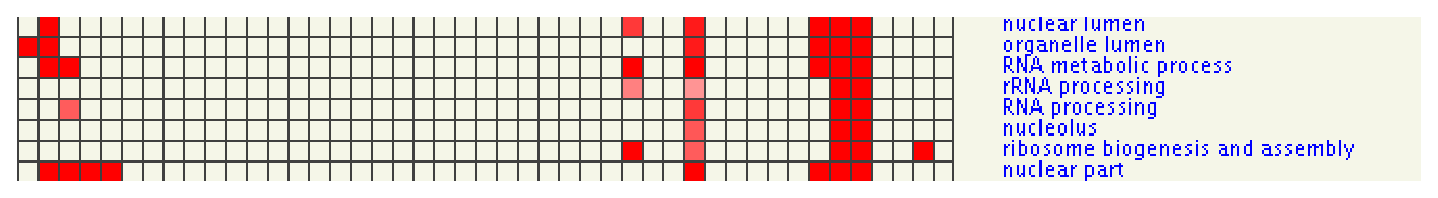
\includegraphics[bb=0 0 674 79, scale=0.5]{images_only/semisup/results/analysis/img_stress_only/1.eps}
\label{fig:stress_only_enrich_1}
}
\subfigure[Section of the image showing significant enrichment]{
\includegraphics[bb=0 0 775 967, scale=0.4]{images_only/semisup/results/analysis/img_stress_only/2.eps}
\label{fig:stress_only_enrich_2}
}
\label{fig:stress_only_enrich}
\caption{Sections of the image showing significant enrichment in Stress only dataset. }
\end{figure}

\begin{figure}[p]
\centering
\subfigure[Section of the image showing significant enrichment]{
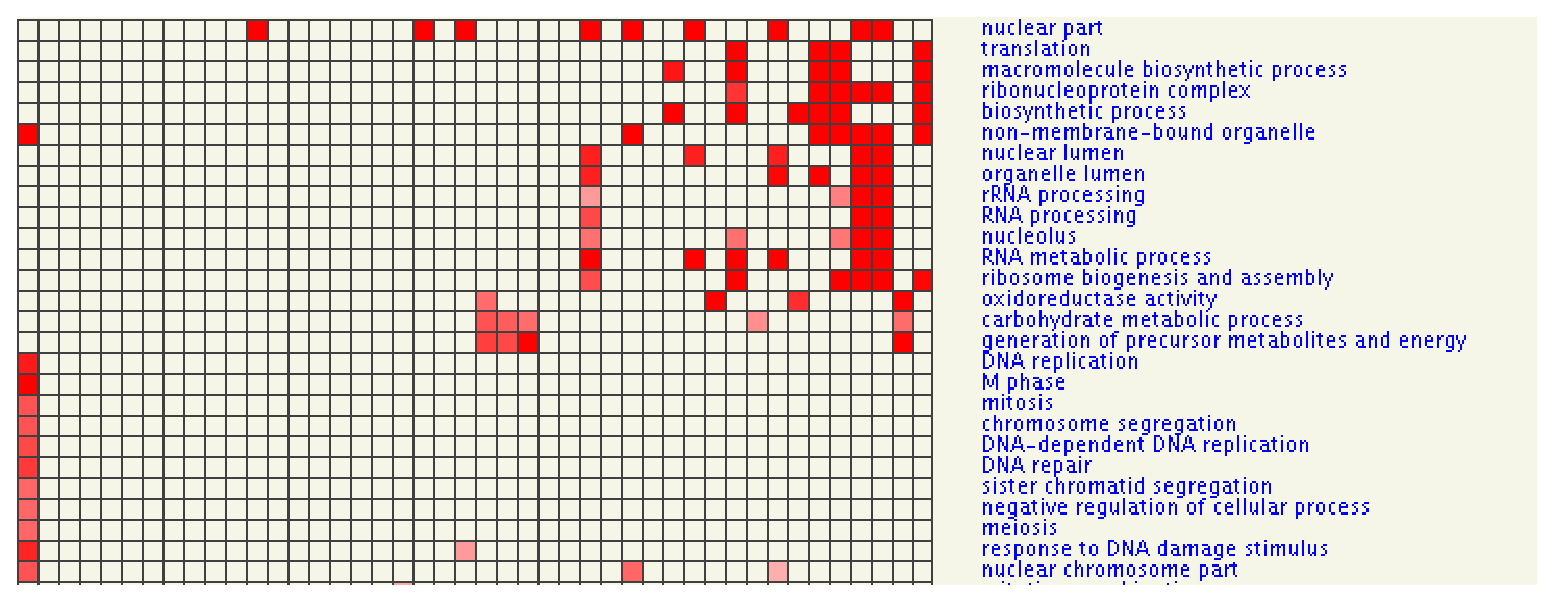
\includegraphics[scale=0.5]{images_only/semisup/results/analysis/img_stress_chip/1.eps}
\label{fig:stress_chip_enrich_1}
}
\subfigure[Section of the image showing significant enrichment]{
\includegraphics[scale=0.4]{images_only/semisup/results/analysis/img_stress_chip/2.eps}
\label{fig:stress_chip_enrich_2}
}
\label{fig:stress_chip_enrich}
\caption{Sections of the image showing significant enrichment in Stress dataset combined with knowledge from ChIP-chip dataset. }
\end{figure}

\begin{figure}[p]
\centering
\subfigure[Section of the image showing significant enrichment]{
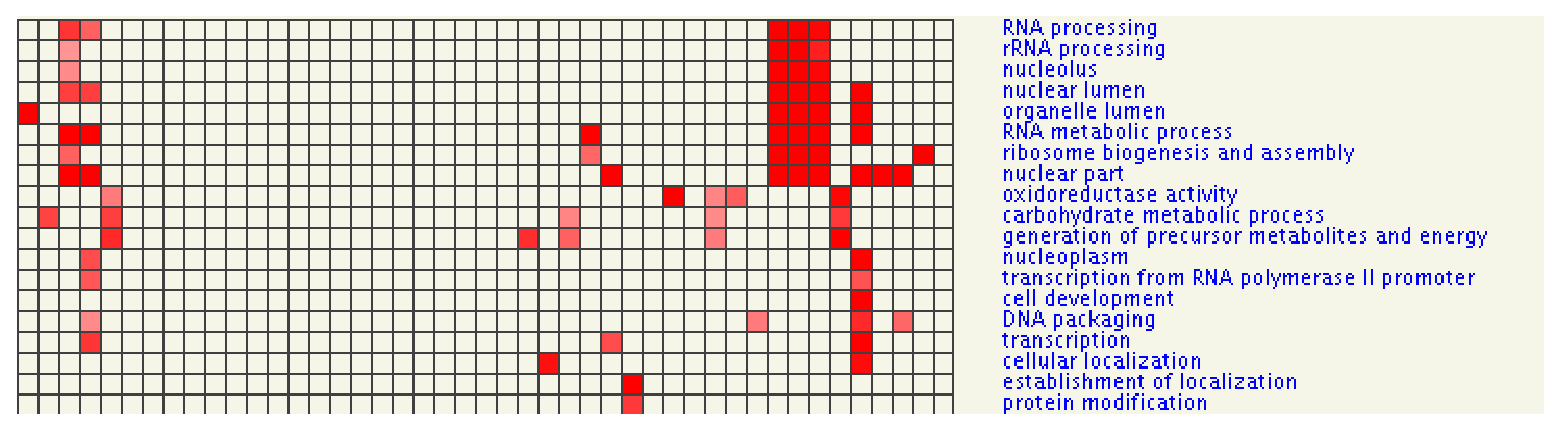
\includegraphics[scale=0.5]{images_only/semisup/results/analysis/img_stress_ppi/1.eps}
\label{fig:stress_ppi_enrich_1}
}
\subfigure[Section of the image showing significant enrichment]{
\includegraphics[scale=0.4]{images_only/semisup/results/analysis/img_stress_ppi/2.eps}
\label{fig:stress_ppi_enrich_2}
}
\label{fig:stress_ppi_enrich}
\caption{Sections of the image showing significant enrichment in Stress dataset combined with knowledge from PPI dataset. }
\end{figure}

\begin{figure}[p]
\centering
\subfigure[Section of the image showing significant enrichment]{
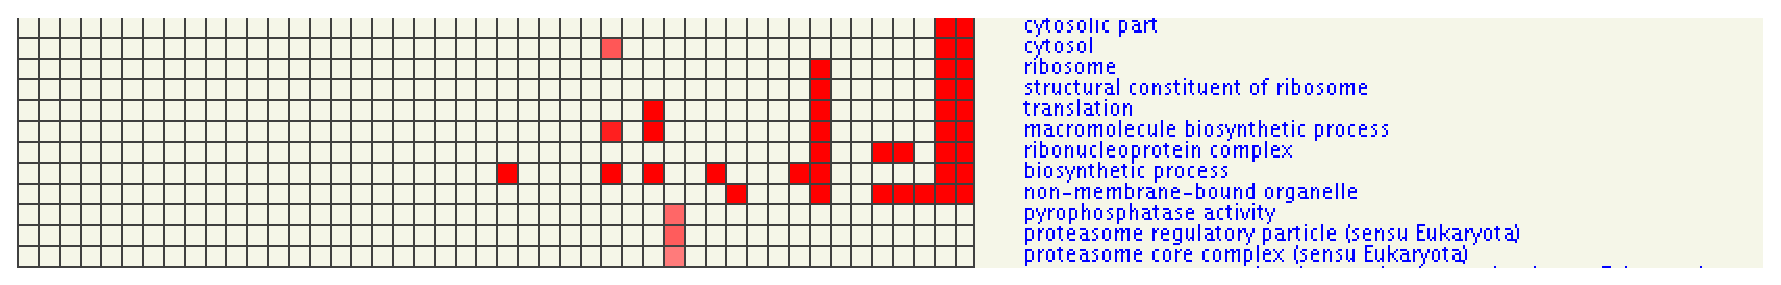
\includegraphics[scale=0.5]{images_only/semisup/results/analysis/img_stress_yt/1.eps}
\label{fig:stress_yt_enrich_1}
}
\subfigure[Section of the image showing significant enrichment]{
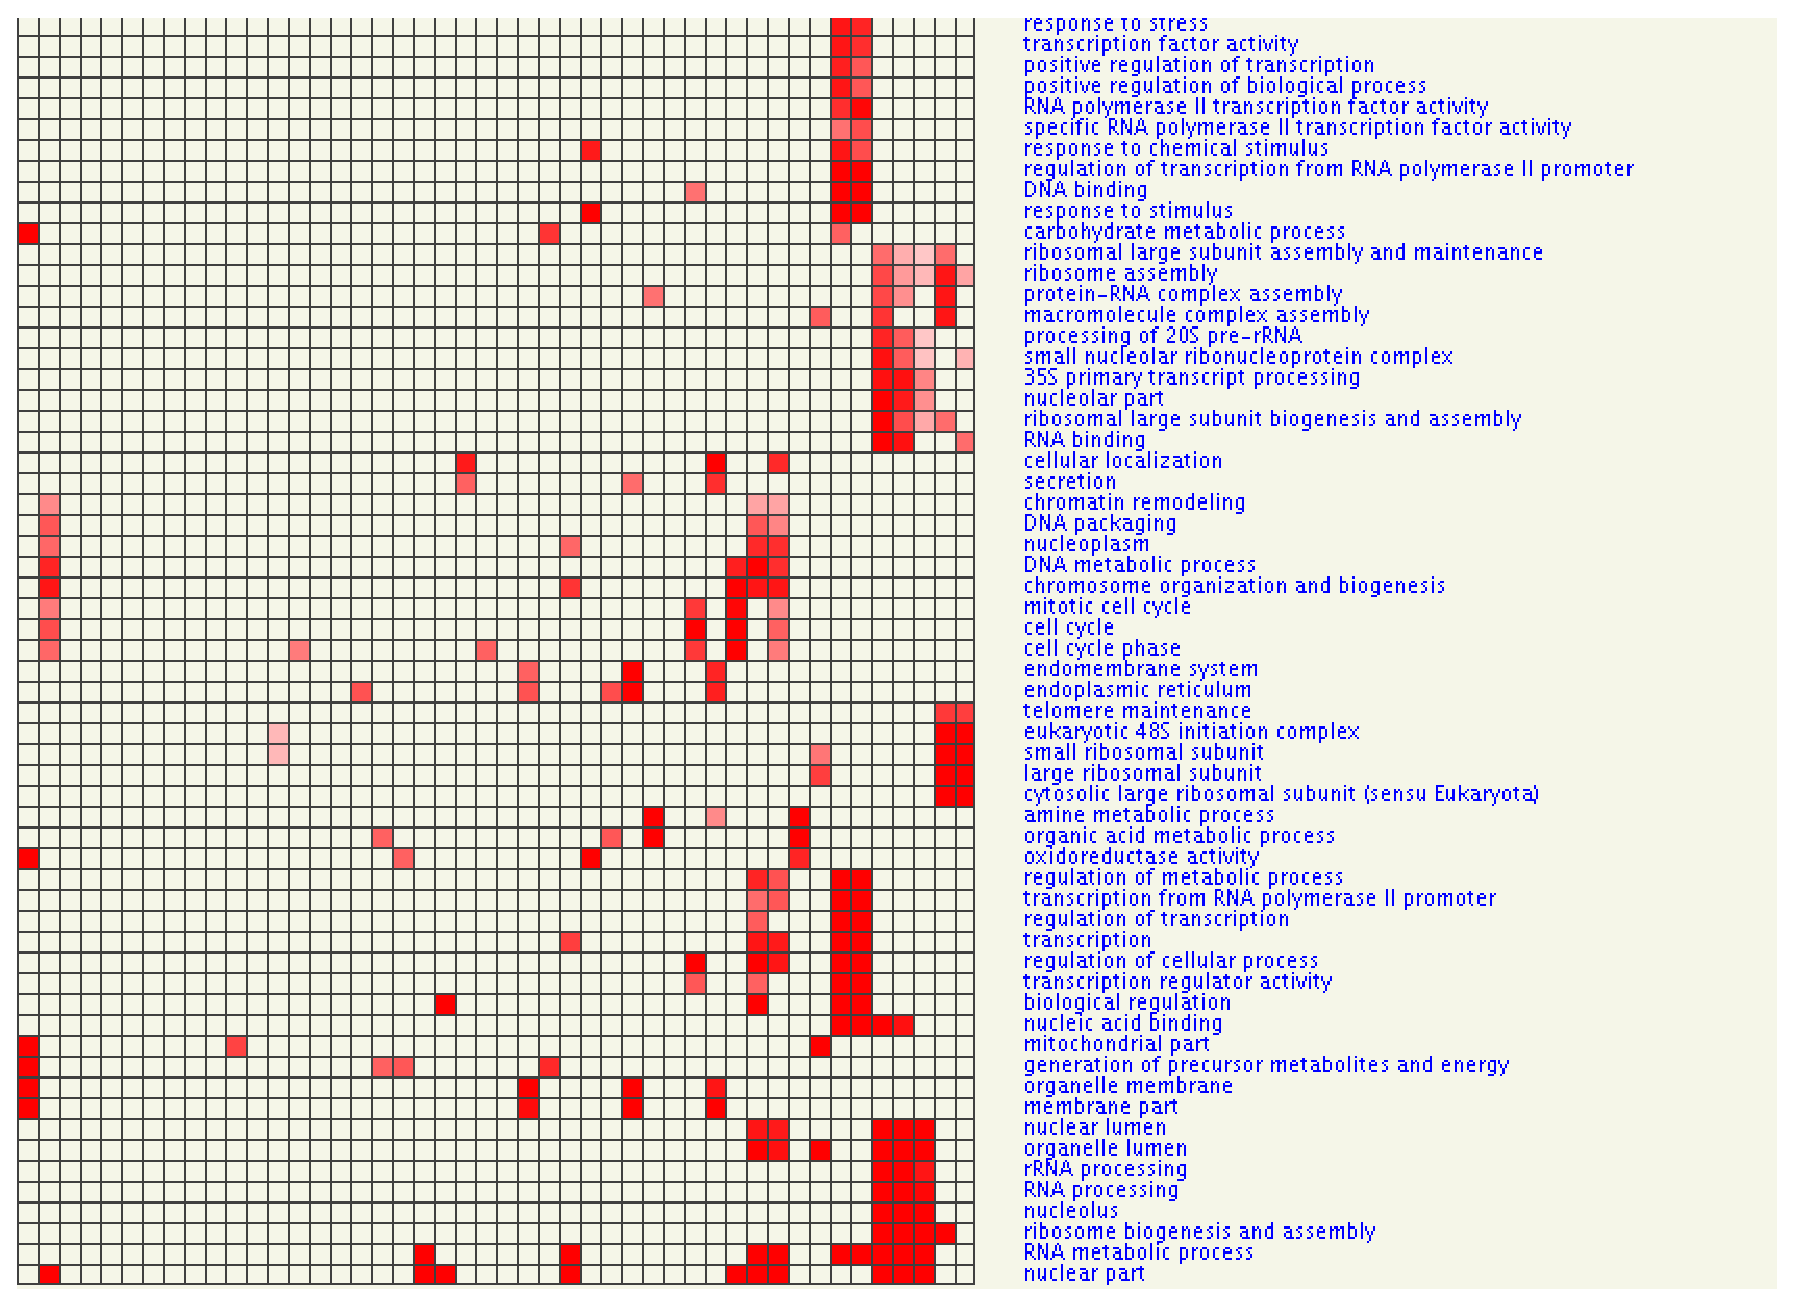
\includegraphics[scale=0.4]{images_only/semisup/results/analysis/img_stress_yt/2.eps}
\label{fig:stress_yt_enrich_2}
}
\label{fig:stress_yt_enrich}
\caption{Sections of the image showing significant enrichment in Stress dataset combined with knowledge from Yeastract dataset. }
\end{figure}

\subsubsection{Stress vs Stress and PPI}

Biological processes like RNA metabolism, RNA binding, rRNA processing, RNA processing, 35S primary transcription, nucleic acid binding, DNA metabolic process are common 
significant enrichments observed in the both the datasets. When combined with PPI dataset, it also shows significant enrichment for processes like oxidoreductase activity, 
transcription from RNA polymerase II promoter, transcription, regulation of transcription, regulation of metabolic process, developmental process, cell cycle phase, 
mitotic cell cycle, biological regulation, regulation of cellular process and chromosome organization and biogenesis when compared to Stress dataset alone. These genes associated to these
biological processes could be studied further to find relationships among them.

\subsubsection{Stress vs Stress and ChIP-chip}

Apart from processes like RNA processing, RNA metabolic process, ribosome biogenesis, macromolecule biosynthetic process and translation which are common enrichment observed 
in the two data sets, the Stress dataset when combined with ChIP-chip dataset also shows significant enrichment for processes like biosynthetic process, cellular localization, 
hydrolase activity, amine metabolic process, amine biosynthetic process, chromosome organization and biogenesis and regulation of cellular process.

\subsubsection{Stress vs Stress and Yeastract}

Translation, macromolecule biosynthetic process, biosynthetic process, 35S primary transcript processing, ribosomal biogenesis and assembly, RNA binding, DNA metabolic process, 
nucleic acid bing, rRNA processing, RNA processing and RNA metabolic process are a few of the common enriched processes observed between Stress and Stress Yeastract. 
However, processes like response to stress, transcription factor activity, positive regulation of transcription, positive regulation of biological process, 
RNA polymerase II transcription factor activity, response to chemical stimulus, regulation of transcription from RNA polymerase II promoter, 
DNA binding, response to stimulus, cellular localization, chromosome organization and biogenesis, mitotic cell cycle, cell cycle, cell cycle phase, 
telomere maintenance, amine metabolic process, organic acid metabolic process, oxidoreductase activity, regulation of metabolic process, regulation of transcription, transcription, 
regulation of cellular process, transcription of regulator activity and biological regulation are other significant enrichment observed only 
in Stress Yeastract as compared to Stress dataset.

\begin{figure}[p]
\centering
\subfigure[Section of the image showing significant enrichment]{
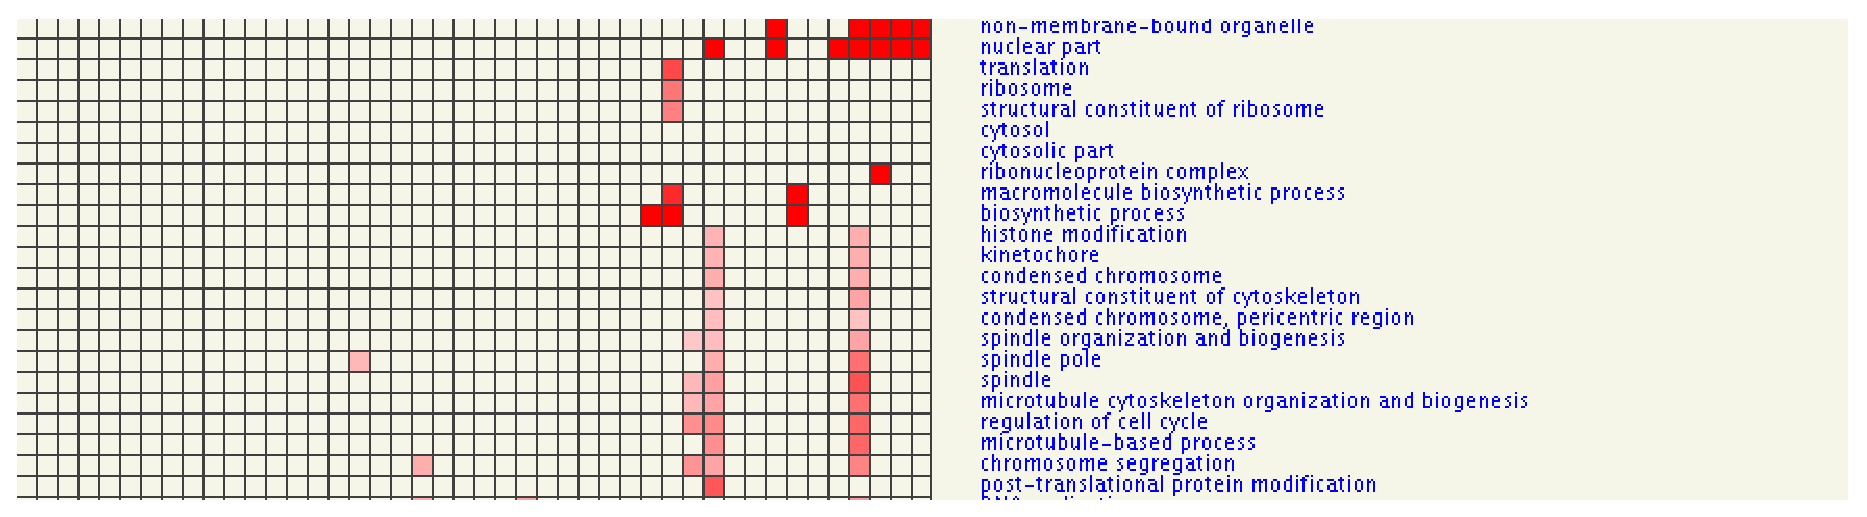
\includegraphics[scale=0.5]{images_only/ec2machine/semisup/results/analysis/ccycle_only/1.eps}
\label{fig:ccycle_only_enrich_1}
}
\label{fig:ccycle_only_enrich}
\caption{Sections of the image showing significant enrichment in Cell-cycle dataset. }
\end{figure}

\begin{figure}[p]
\centering
\subfigure[Section of the image showing significant enrichment]{
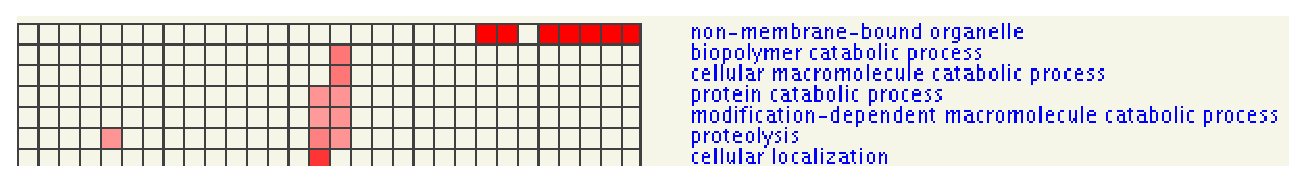
\includegraphics[scale=0.5]{images_only/ec2machine/semisup/results/analysis/ccycle_ppi/1.eps}
\label{fig:ccycle_ppi_enrich_1}
}
\subfigure[Section of the image showing significant enrichment]{
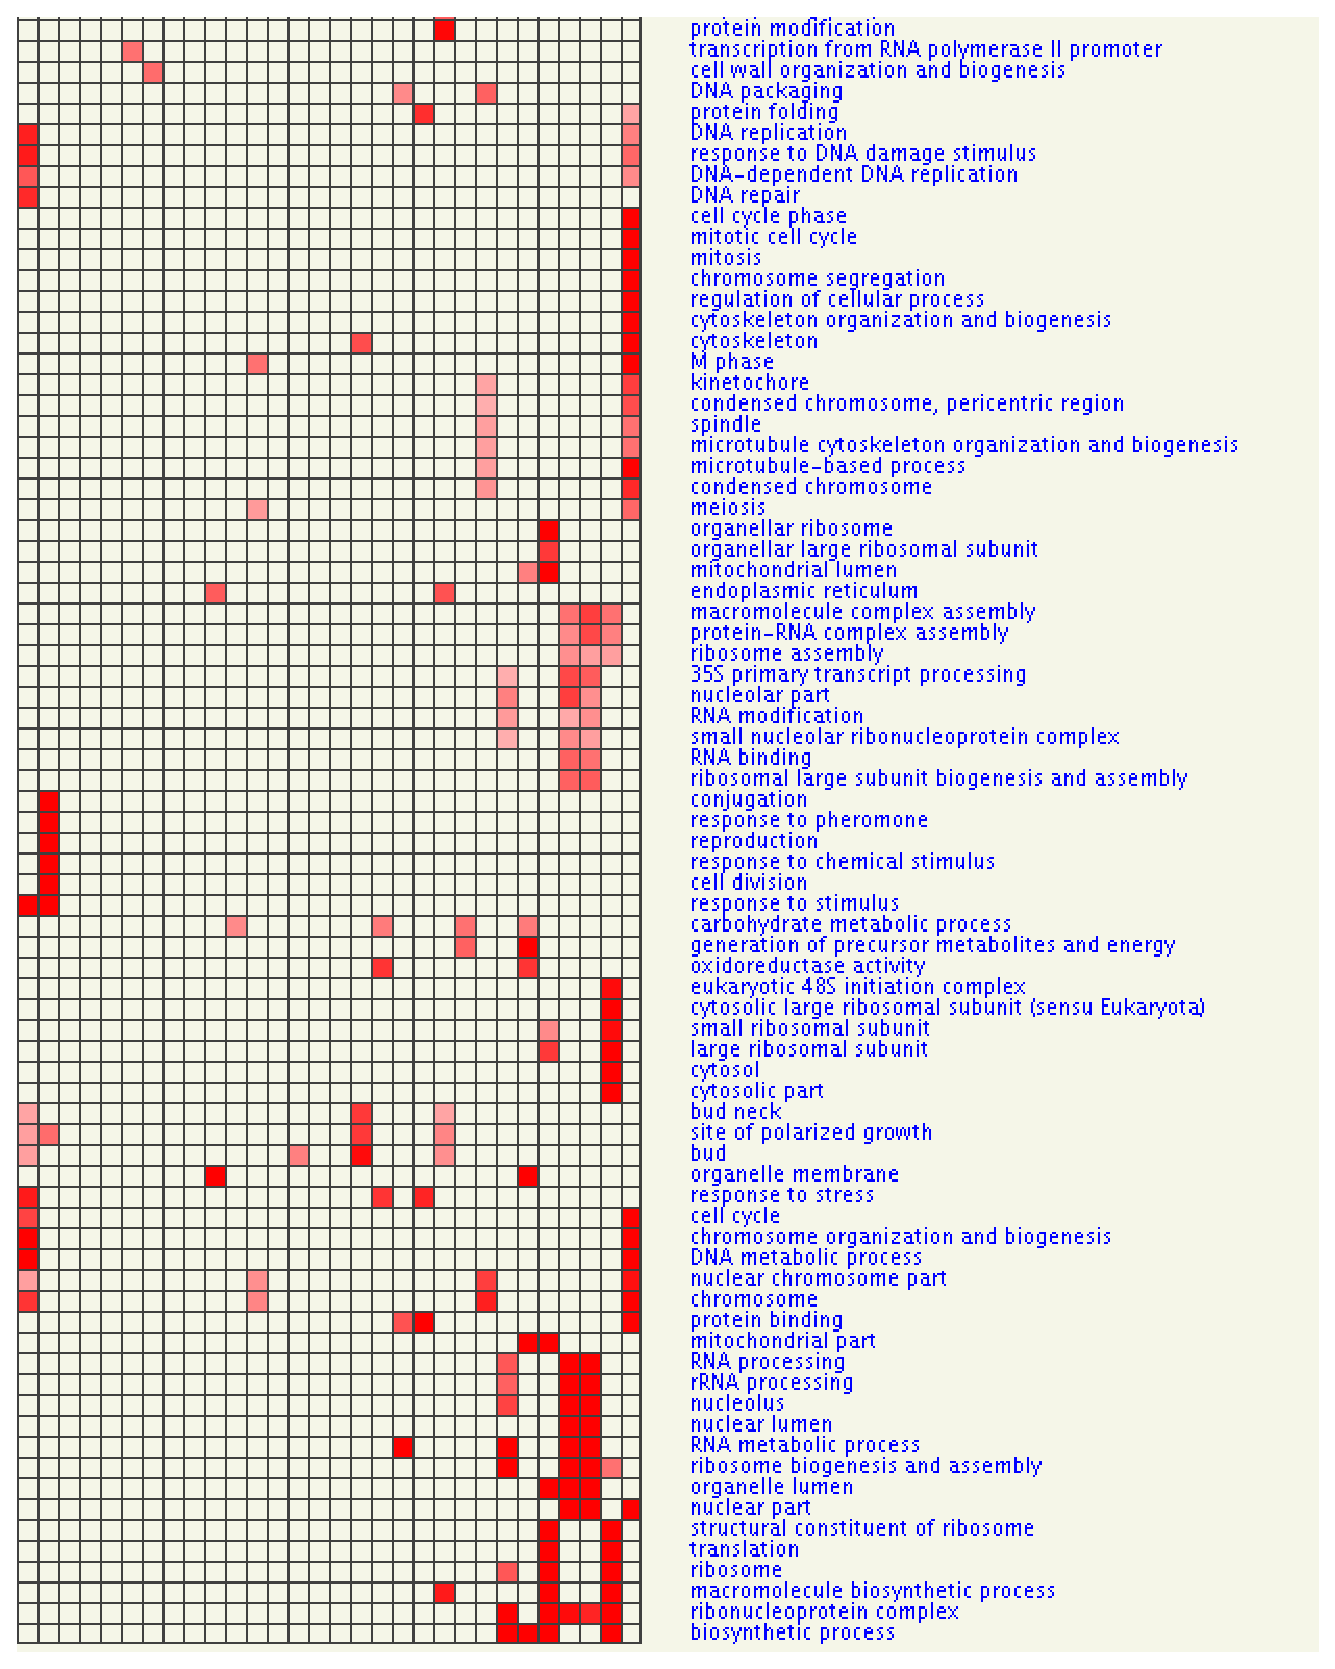
\includegraphics[scale=0.5]{images_only/ec2machine/semisup/results/analysis/ccycle_ppi/2.eps}
\label{fig:ccycle_ppi_enrich_2}
}
\label{fig:ccycle_ppi_enrich}
\caption{Sections of the image showing significant enrichment in Cell-cycle dataset combined with knowledge from PPI dataset. }
\end{figure}

\begin{figure}[p]
\centering
\subfigure[Section of the image showing significant enrichment]{
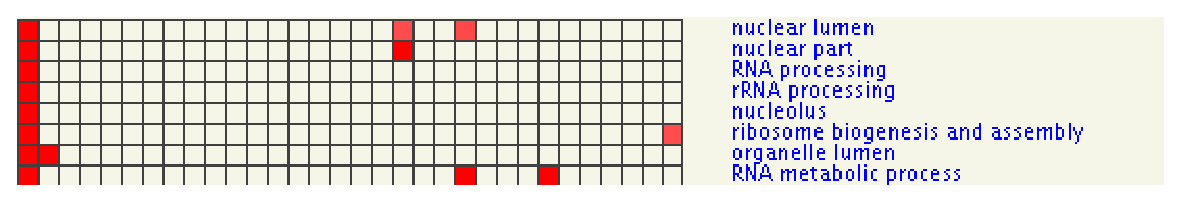
\includegraphics[scale=0.5]{images_only/ec2machine/semisup/results/analysis/ccycle_chip/1.eps}
\label{fig:ccycle_chip_enrich_1}
}
\subfigure[Section of the image showing significant enrichment]{
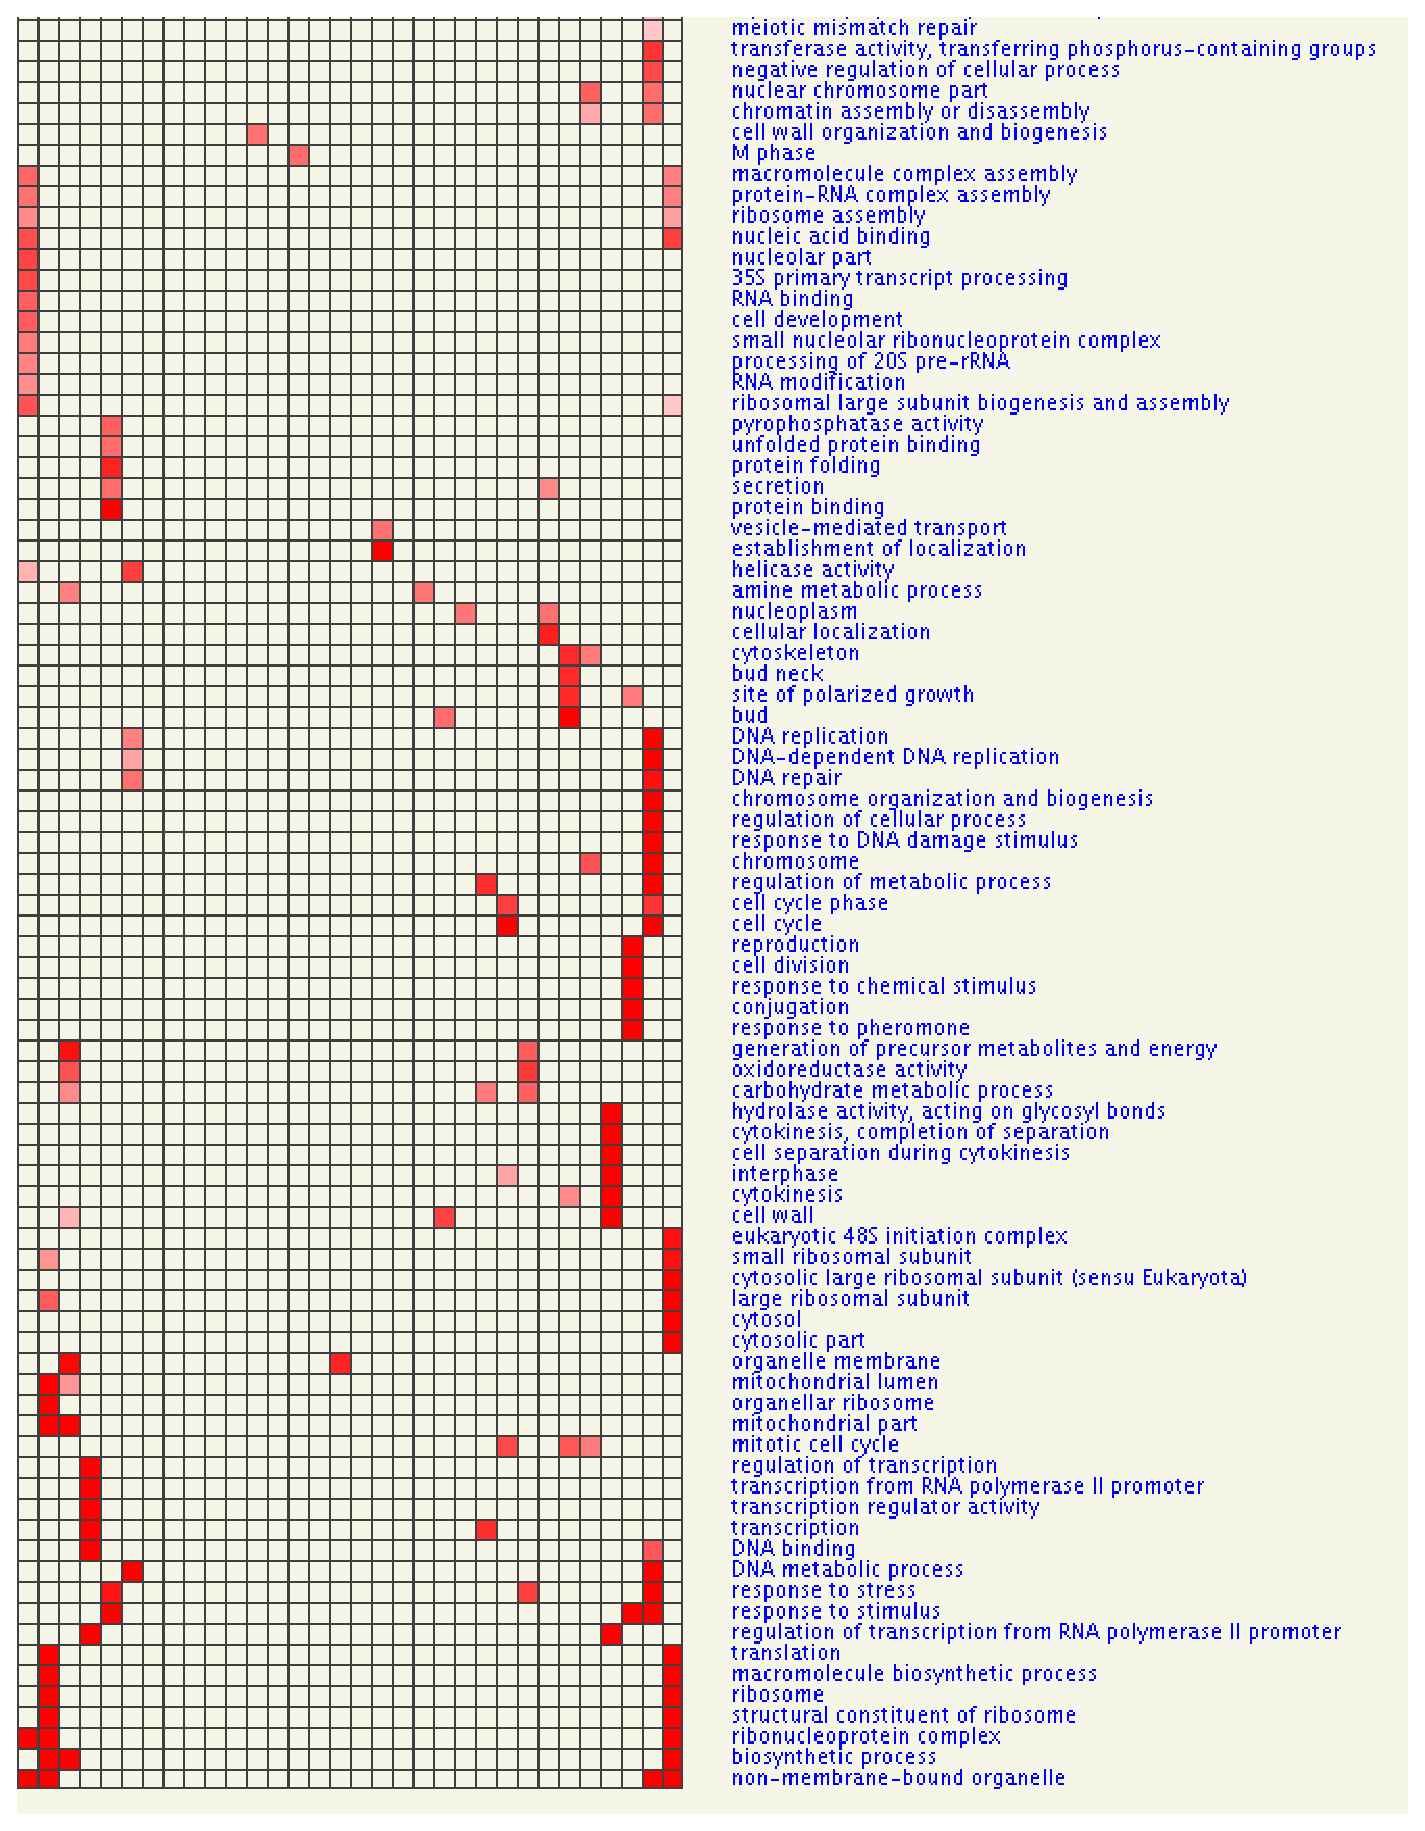
\includegraphics[scale=0.5]{images_only/ec2machine/semisup/results/analysis/ccycle_chip/2.eps}
\label{fig:ccycle_chip_enrich_2}
}
\label{fig:ccycle_chip_enrich}
\caption{Sections of the image showing significant enrichment in Cell-cycle dataset combined with knowledge from ChIP-chip dataset. }
\end{figure}


\begin{figure}[p]
\centering
\subfigure[Section of the image showing significant enrichment]{
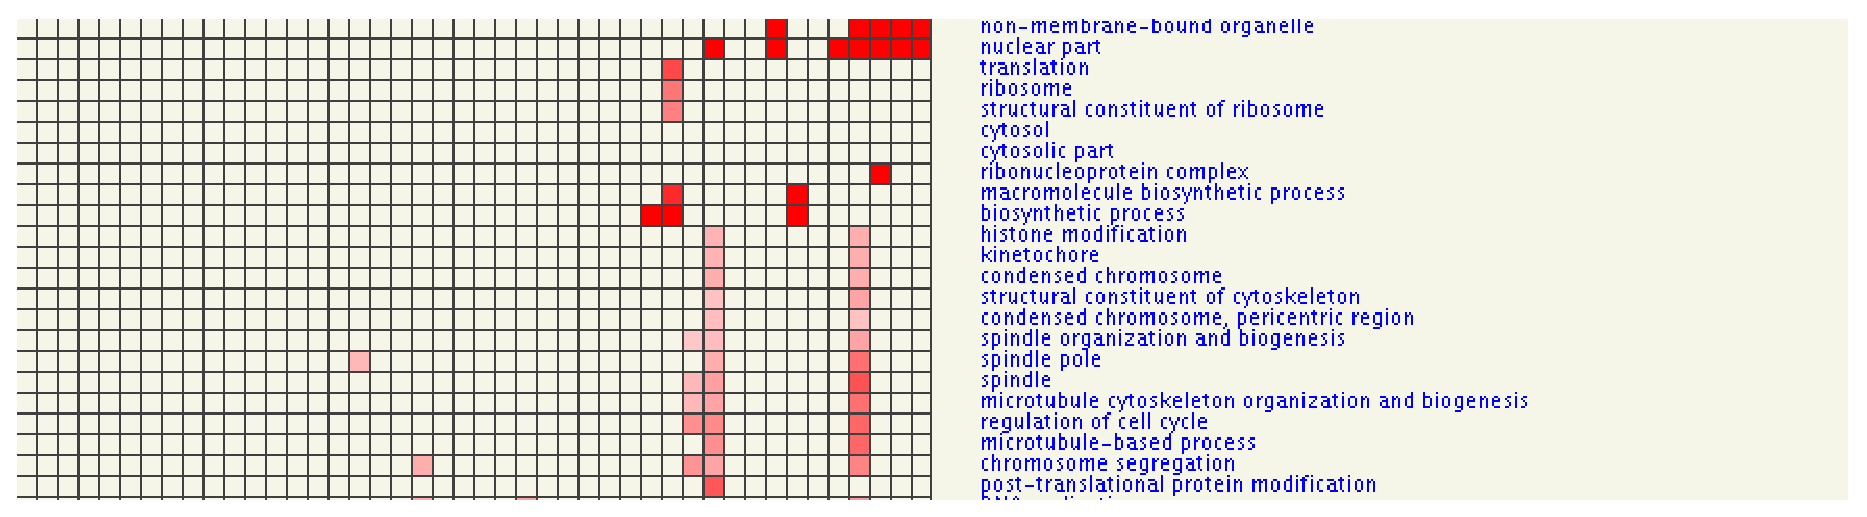
\includegraphics[scale=0.5]{images_only/ec2machine/semisup/results/analysis/ccycle_only/1.eps}
\label{fig:ccycle_yt_enrich_1}
}
\label{fig:ccycle_yt_enrich}
\caption{Sections of the image showing significant enrichment in Cell-cycle dataset combined with Yeastract dataset. }
\end{figure}

\subsubsection{Cell-Cycle vs Cell-Cycle and ChIP-chip}

DNA metabolic process, translation, macromolecule biosynthetic process and biosynthetic process are found to be common to the Cell-Cycle dataset before and after combination with the 
ChIP-chip dataset. After combination we see significant enrichment for response to stress, response to stimulus and regulation of transcription from polymerase II when compared 
to Cell-Cycle data set alone.

\subsubsection{Cell-Cycle Vs Cell-Cycle and PPI}

The DNA metabolic process, RNA processing, rRNA processing, the RNA metabolic process, macromolecule biosynthetic process, biosynthetic process and translation are 
some of the common enriched processes observed in both the data sets. Besides these, Cell-Cycle when combined with the PPI dataset also showed significant enrichment for 
oxidoreuctase activity, response to stress, cell-cycle, chromosome organization and biogenesis and protein binding 
when compared to the Cell Cycle data set alone. We observe that even though
cell-cycle processes were not accentuated earlier, after combination with the PPI dataset, they shows up prominently. 

\subsubsection{Cell-Cycle vs Cell-Cycle and Yeastract}

The RNA binding, 35S primary transcription process, RNA processing, rRNA processing, RNA metabolic process, macromolecule biosynthetic process, 
translation and biosynthetic process are the common significant enrichment sites observed in the Cell-Cycle dataset both before and after combination with the Yeastract dataset. 
The Cell-Cycle dataset when combined with the Yeastract dataset also showed enrichment significantly for RNA modification, response to stimulus, mitotic cell cycle 
and DNA metabolic process when compared to Cell Cycle data set alone. 

\begin{comment}
\section{Results}
\begin{table}[t]
\centering
\scalebox{0.9}{
\begin{tabular}{@{\extracolsep{\fill}}|p{0.75in}|p{0.90in}|p{0.70in}|p{0.70in}|p{0.65in}|p{0.70in}|p{0.70in}|p{0.65in}|}
\hline
\multicolumn{2}{|c|}{Constraint Source} & \multicolumn{6}{|c|}{Mean Enrichment}\\ \cline{1-8}
& p-value cutoffs (no. of constraints) & \multicolumn{3}{|c|}{across all terms} & \multicolumn{3}{|c|}{for top 50 terms}\\ \cline{3-8}
       & & Before integration &  After integration & Percent gain & Before integration &  After integration & Percent gain\\
\hline
\multirow{7}{*}{ChIP-chip}& & & & & & & \\ 
& 0.0001 (544)  &  8.101  &  9.029  &  11.457 & 11.057  &  12.266  &  10.938 \\ 
& 0.0005 (846)  &  8.101  &  8.923  &  10.151 & 11.057  &  13.324  &  20.500 \\ 
& 0.001 (1053)  &  8.101  &  8.404  &  3.735  & 11.057  &  12.546  &  13.465 \\ 
& 0.005 (1959)  &  8.101  &  7.617  &  -5.974 & 11.057  &  10.831  &  -2.048 \\ 
& 0.01 (2776)    &  8.101  &  8.613  &  6.323  & 11.057  &  12.206  &  10.389 \\ 
& 0.05 (7407)    &  8.101  &  7.927  &  -2.148 & 11.057  &  10.826  &  -2.088 \\ 
& 0.1 (12579)     &  8.101  &  7.692  &  -5.047 & 11.057  &  10.610  &  -4.045 \\ \hline
PPI  & All (442) &  8.101  &  7.849  &  -3.116 & 11.057  &  11.462  &  3.664  \\ \hline
Yeastract & All (8644) &  8.101  &  7.325  &  -9.579 & 11.057  &  10.695  &  -3.271 \\

\hline 
\end{tabular}
}
\caption{Stress microarray dataset: Comparison of mean p-values of enriched GO terms before and after supervision}
\label{tab:stress:semisup_mean_pvals}
\end{table}

\begin{table}[t]
\centering
\scalebox{0.9}{
\begin{tabular}{@{\extracolsep{\fill}}|p{0.75in}|p{0.94in}|p{0.70in}|p{0.70in}|p{0.65in}|p{0.70in}|p{0.70in}|p{0.65in}|}
\hline
\multicolumn{2}{|c|}{Constraint Source} & \multicolumn{6}{|c|}{Mean Enrichment}\\ \cline{1-8}
& p-value cutoffs (no. of constraints)& \multicolumn{3}{|c|}{across all terms} & \multicolumn{3}{|c|}{for top 50 terms}\\ \cline{3-8}
       & & Before integration &  After integration & Percent gain & Before integration &  After integration & Percent gain\\
\hline
\multirow{7}{*}{ChIP-chip}& & & & & & & \\ 
& 0.0001 (681) &   7.167 &   7.412 &   3.419	& 9.411 & 10.108 & 7.407 \\ 
& 0.0005 (1032) &   7.167 &   7.156 &   -0.158 & 9.411 & 9.547  & 1.442  \\
& 0.001 (1288)  &   7.167 &   7.124 &   -0.610 & 9.411 & 9.578  & 1.773  \\
& 0.005 (2442)  &   7.167 &   7.228 &   0.842	& 9.411 & 8.842  & -6.043 \\
& 0.01 (3505)   &   7.167 &   7.713 &   7.617	& 9.411 & 10.305 & 9.496  \\
& 0.05 (9713)   &   7.167 &   7.997 &   11.576 & 9.411 & 10.453 & 11.071 \\
& 0.1 (17055)    &   7.167 &   8.085 &   12.809 & 9.411 & 10.065 & 6.951  \\ \hline
PPI       & All (1129) &   7.167 &   6.784 &   -5.349 & 9.411 &   9.825  &   4.399 \\ \hline 
Yeastract & All (9717) &   7.167 &   7.392 &   3.134  & 9.411 &   10.155 &   7.910 \\
\hline 
\end{tabular}
}
\caption{Cell-cycle microarray dataset: Comparison of mean p-values of enriched GO terms before and after supervision}
\label{tab:ccycle:semisup_mean_pvals}
\end{table}
\end{comment}

\section{Related Work and Discussion}
\subsection{Constrained clustering}
The concept of applying prior knowledge in the form of constraints to clustering algorithms is not new. Initial \textit{supervised} clustering algorithms were modifications of traditional ones and ensured that the resulting clusters had to satisfy the applied constraints. One of the first papers in this area by \citet{bradley00constrained} proposed a constrained version of the famous \textit{k-means} \citep{MacQueen67kmeans} clustering algorithm by posing the problem in terms of minimum cost network flows. Their objective behind adding the constraints was to assign a certain minimum number of points to each cluster. \citet{tung2001constraint} have done a systematic study of various constrained clustering algorithms. \citet{basu2008constrained} is a recent book on constrained clustering.

\subsection{Semi-supervised clustering}
While constrained clustering algorithms work towards satisfying known constraints, other distance based clustering algorithms were developed in which the metric that a clustering algorithm uses in order to calculate distance between a pair of data-points was modified by incorporating constraints from other sources of data. These were the first \textit{semi-supervised} clustering algorithms. They did not enforce the constraints, but used the constraints to provide guidance in the cluster formation process. This is the crucial difference between a \textit{supervised} and a \textit{semi-supervised} clustering algorithm. In the former, the constraints are derived from known ground truth and have to be satisfied, whereas in the latter, the constraints are additional sources of information but are considered noisy and hence not necessarily exactly correct. This is a characteristic of the DNA-binding, PPI and TF-gene interactions data that we use for deriving our constraints, and also our justification for using the semi supervised algorithm. 

\citet{klein2002frominstance} used the concept of ``must-link'' and ``can-not link'' constraints on hierarchical agglomerative clustering \citep{jain1988algorithms}. 
They reported that it improved upon earlier constrained clustering algorithms and required a much smaller number of constraints for similar accuracy. 
According to them constraints suggest space-level generalizations beyond their instance-level assertions. In other words, if a point A is linked to another point B, 
then A should also probably be linked to points that are near B and \textit{vice-versa}. They used this idea to \textit{propagate} constraints. \citet{basu2004probabilistic} have 
proposed a probabilistic model for semi-supervised clustering based on \acp{HMRF} that provides a more principled framework for incorporating supervision. It combines the constraint based and distance based approached into a single unified model.
 
Our technique is likewise based on the concept of using the constraints obtained from one dataset in order to modify the similarity value that is obtained from another dataset. The key difference is that while all the previous work has used this principal to do clustering in some feature space, our technique uses the modified similarity values to cluster in spectral space (spectral clustering). 

\subsubsection{Spectral clustering}
The field of spectral clustering was started by \citet{donath1973lower} who came up with the idea of constructing graph partitions using the eigenvectors of an adjacency matrix. It has generated a lot of interest in recent years \citep{shi00normalized,ng2001onspectral} in clustering related research and has been applied from \textit{object retrieval} \citep{jain06spectral} to \textit{brain surface flattening} \citep{angenent99laplace}. A nice review of this subject and its relation to other related topics can be found in \citet{luxberg2006tutorial_spectral} and an upcoming\footnote{to be published in Feb 2010} book by \citet{ding2008spectral}.

As we have discussed earlier, spectral clustering works on similarity matrices. In that respect, it is similar to \textit{multi-dimensional scaling} or in general, the broader class of \textit{metric multidimensional scaling} \citep{deleeuw2005mds} algorithms which also operate on a similarity matrix and are useful for visualization of high dimensional data by mapping it to lower dimensions. The key difference between these and spectral clustering is that while they operate in the feature space, spectral clustering works in the spectral space. Spectral clustering has close relations to the field of non-linear dimensionality reduction techniques like \textit{manifold learning} \citep{saul2006smd, haifang2006manifold} and semi-supervised learning \citep{grira2005unsupsurvey}. \citet{nadler06fundamental} have discussed the fundamental limitations of spectral clustering. \citet{dhillon05unified} have shown the equivalence between kernel k-means \citep{johnshaw2004kernelmethods} and spectral clustering. This result gains importance when the similarity matrix is too large for eigen-decomposition and iterative techniques need to be used. 

Even before the recent interest in spectral clustering, a matrix formalism has been used to describe the functional states of transcriptional regulatory systems. \citet{gianchandani2006matrix} used such a model to characterise the properties of \acp{TRS} and facilitate the computation of the transcriptional state of the genome under any given environmental conditions. 

One of the first applications of spectral clustering to bioinformatics was by \citet{kluger2003spectral} who used it to simultaneously clusters genes and conditions (biclustering) for various cancer datasets. In a cancer context, the clusters correspond to genes that are markedly up or down regulated in patients with particular types of tumors. They present a number of variants of the approach, depending on whether the normalization over genes and conditions is done independently or in a coupled fashion. They analysed publicly available cancer expression data sets, and examined the degree to which the approach is able to identify clusters. They have also compared the performance against a number of reasonable benchmarks (e.g., direct application of SVD or normalized cuts to raw data). \citet{speer05spectral} used spectral clustering to cluster Gene Ontology terms to find sets of genes that might be functionally related. They used an information theoretic measure borrowed from text mining, where it had been used to calculate semantic similarities between words, to calculate the similarity values between the terms of the Gene Ontology.

\subsubsection{Semi-supervised spectral clustering}
\citet{kamvar03spectral} propose an algorithm for classification called \textit{spectral classification} which modifies the similarity matrix to 1 if the known training data 
belong to the same class and 0 otherwise. The similarity matrix is subject to eigen-decomposition and then classification is done in the spectral space. The advantage of doing this is that they can use labelled data (provides class constraints) as well as unlabelled data (similarity computation). They report better performance than the \textit{naive Bayes} classifier in classifying newsgroups. They have also proposed a constrained spectral clustering with must-link and cannot-link constraints along with an additive normalized laplacian \citep{fiedler1975property} and used it for classification. The results and the comparison with other algorithms for this is not systematic and clearly presented which makes it difficult to judge its performance. 

\citet{brian_semisupgraph2005} proposed a semi-supervised version of the kernel k-means algorithm. The difference between our formulation and theirs is that after modifying the similarity matrix we use spectral clustering while they have used kernel k-means algorithm. They argue that this might be better for larger datasets where eigenvalue computation might be computationally expensive whereas kernel k-means being a iterative algorithm, doesn't face this problem. This is true but the drawback with kernel k-means is that like k-means it can get stuck in local optima while spectral techniques always try to approximate the global optimum.

Most algorithms discussed till now rely critically on a good metric over their inputs. If a clustering algorithm fails to find clusters that are meaningful, then the recourse usually is to manually tweak the metric until sufficiently good clusters are found. \citet{xing2003metric} proposed an algorithm that, given examples of similar (and, if desired, dissimilar) pairs of points, \textit{learns} a distance metric that respects these relationships. They also demonstrate that the learned metrics can be used to significantly improve clustering performance. 

\subsection{Co-clustering}
This is a related and overlapping technique where two or more sources of data are combined. The key difference from semi-supervised or constrained clustering is that in co-clustering, one dataset is not used to guide the other. Rather, both the datasets are combined with equal or varying weights by combining their distance metrics to come up with a new one which is then used for clustering. We will see a detailed discussion and review in the next chapter.

\section{Conclusion}

We have proposed a technique to integrate diverse datasets where one is acting as a source of supervision on the clustering of the other. 
As part of this, we have investigated whether constraints are useful at all in order to retrive the original clustering from a noisy version of the original dataset. We also investigated 
two methods for determining the best Gaussian kernel to obtain the affinity matrix from the data. Further, we have used a validation method which scores the resulting gene clusters 
by reference to a third type of data (Gene Ontology). Our results indicate that semi-supervised spectral clustering leads to improved biological significance if the datasets from 
which known facts are extracted is not widely varying from the datasets on which they are applied.  

Since our technique is quite generic, in future, our work can be extended by using other sources of prior knowledge, for example the similarity between 
the promoter sequences of genes. In the next chapter, we propose a technique where instead of creating definite constraints, we extract similarities from graphs of interactions and 
then integrate the datasets. It is based on the principle of maximizing the entropy of the resulting matrix. 

One of the shortcomings of this research is that it is known that gene regulation is a very condition specific activity and hence the expression values that 
we observe are a result of regulation happening at one particular time. However, the datasets that we have used are from different conditions. 
The microarray datasets as well as the DNA-binding, PPI and Yeastract datasets were not experimentally observed at the same time or even by the same researchers. 
This is also a fundamental limitation of the underlying experimental techniques, since microarrays themselves do not represent a single time point, 
but rather the integration of gene activity over a time period. Moreover, knowledge about gene modules is not complete and this hinders the validation process. 

